\chapter{Code Implementation for Sirius}\label{chap:code_studies}
This chapter is dedicated to the discussion about LOCO method implementation for Sirius storage ring, using Python as the programming language. Some tests were performed to check the reliability of the implemented code and also to understand the particularities related to the application on Sirius.

\section{Accelerator Physics Codes}
The Python frameworks mentioned in Section~\ref{sec:master_obj} for the accelerator physics studies are related to the accelerator modelling, the so-called tracking simulations and optics calculations. The corresponding packages developed and currently used by the LNLS~\gls{fac} are described as follows.

\begin{description}
    \item[PyModels:] Python modelling for the accelerator where each element is defined with several properties: device type (magnet, diagnostic, etc), length, strength, pass method, etc. The element pass method is the rule that the tracking code uses to evolve in time the particle's phase-space coordinates. The code access is open and it contains versions for the models of the Sirius accelerators:~\gls{linac}, transport lines, booster and storage ring~\cite{pymodels}
    \item[TrackCpp:] tracking code implemented in C++ language. With the accelerator model, the particle dynamics can be numerically studied using the transfer concatenated maps that are applied to the particles coordinates. Each lattice element can be represented by a map $\mathbf{T}(s|s_0)$ and it effects the particle coordinates $\vec{r}_0 = \left(x_0, x'_0, y_0, y'_0, z_0, \delta_0\right)$ at $s_0$ by changing the coordinates to $\vec{r} = \mathbf{T}(s|s_0)\vec{r}_0$. Regarding the linear dynamics, the correspondence between the matrix formalism (linearized maps) and the analytical description presented in Chapter 2 was developed by Courant \& Snyder in~\cite{CourantSnyder1958}. The map approach is extremely useful for numerical calculations and its linearized form takes advantage on linear algebra conveniences, for example the fact that the transformation compositions are translated simply as matrix multiplications. For circular accelerators, the whole lattice transformation, called the one-turn map, is very useful for deriving global lattice properties, verify long-term stability conditions, obtain fixed points for the map, etc. The one-turn map may include only the linear contributions or non-linear effects. For general tracking code like TrackCpp, explicit symplectic integrators are applied to approximate the solutions of the equations of motions for the particles in the lattice in a sistematic way. TrackCpp is an open-source code and can be accessed in~\cite{trackcpp}.
    \item[PyAccel:] Python integration between the accelerator modelling in PyModels and the structures in C++ implemented in TrackCpp. The package also provides the interface to calculate the optics functions for the model (the Twiss functions), to perform the tracking simulations, to calculate the equilibrium parameters (emittance, bunch length, beam sizes), and other useful information for the beam dynamics studies. With this package is also possible to easily manipulate the model, setting or getting the elements properties. The open code can be accessed in~\cite{pyaccel}.
\end{description}

Since PyAccel can be seen as a ``high-level'' interface for the calculations performed in the background by TrackCpp, the accelerator physics simulations are conducted with the combined use of PyModels and PyAccel packages.
\section{Implementation}
Currently the LOCO code for Sirius is a Python package. This package is imported in a Python script that gathers the necessary input data, starts the fitting process and saves the output. At the time of writing, this script was executed via terminal. The detailed implementation of LOCO Python package is completely open for access in its GitHub Repository website~\cite{locosirius}. A functional and tested code version was obtained during this master's work, however the LOCO code is susceptible to changes and improvements based on the experience acquired during the application in Sirius commissioning and machine studies. The upcoming versions will be constantly updated in the website~\cite{locosirius}, open to the community access.

\subsection{Orbit Response Matrix Calculation}
LOCO method requirements are basically a simulated model for the accelerator and a framework to perform the~\gls{orm} calculations in the model. The numerical tools required for LOCO, such as matrix multiplications and~\gls{svd}, are all covered by \textsc{NumPy}, a Python package largely used in scientific computing. 

PyModels provides the accelerator modelling for Sirius storage ring and the~\gls{orm} calculation was already implemented by LNLS~\gls{fac}, where the transfer matrices between BPMs and correctors are used to obtain the corresponding~\gls{orm} elements. This approach assumes linearity, which is typically a good approximation for small variations in the correctors kicks and orbit distortions. The~\gls{orm} calculation from the transfer matrices also has the advantage of being fast: it takes about $\SI{500}{\milli\second}$ to obtain the Sirius storage ring~\gls{orm} in the available computers used by LNLS~\gls{fac}.

Considering that an origin for the coordinate $s$ is defined, let's assume that the~\gls{bpm} longitudinal position is smaller than the corrector (the~\gls{bpm} is behind the corretor), the general transfer matrix between these two elements is
\begin{equation}
    \begin{bmatrix}
    \Delta x \\
    \Delta x' \\
    \Delta y' \\
    \Delta y'
    \end{bmatrix}_{\mathrm{BPM}}  =
    \begin{bmatrix}
    T_{x, x} & T_{x, x'} & T_{x, y} & T_{x, y'} \\
    T_{x', x} & T_{x', x'} & T_{x', y} & T_{x', y'} \\
    T_{y, x} & T_{y, x'} & T_{y, y} & T_{y, y'} \\
    T_{y', x} & T_{y', x'} & T_{y', y} & T_{y', y'} 
    \end{bmatrix} 
    \begin{bmatrix}
    \Delta x \\
    \Delta x' \\
    \Delta y \\
    \Delta y'
    \end{bmatrix}_{\mathrm{corr}}.
\end{equation}

If the~\gls{bpm} is ahead the corrector, the transfer matrix is actually from the~\gls{bpm} to the corrector, so it is the inverse of transfer matrix that must be used for consistency\footnote{Since the transfer matrices must be sympletic, their determinants are equal to one and the inverse transfer matrices exist.}. Since the corrector strength variation affects only the angles, its obtained that  $\Delta x_{\mathrm{corr}}' = \Delta \theta_x \neq 0$ and $\Delta y_{\mathrm{corr}}' = \Delta \theta_y \neq 0$. The positions are unchanged, $\Delta x_{\mathrm{corr}} = \Delta y_{\mathrm{corr}} = 0$, so the~\gls{orm} elements are obtained as 
\begin{align*}
    M_{xx} = \dfrac{\Delta x_{\mathrm{BPM}}}{\Delta \theta_x} = T_{x, x'}, & \hspace{1cm} M_{xy} = \dfrac{\Delta x_{\mathrm{BPM}}}{\Delta \theta_y} = T_{x, y'}, \\
    M_{yx} = \dfrac{\Delta y_{\mathrm{BPM}}}{\Delta \theta_x} = T_{y, x'}, & \hspace{1cm} M_{yy} = \dfrac{\Delta y_{\mathrm{BPM}}}{\Delta \theta_y} = T_{y, y'}.
\end{align*}

For the uncoupled lattice, the crossed elements are null and the transfer matrix is
\begin{equation}
    \begin{bmatrix}
    \Delta x \\
    \Delta x' \\
    \Delta y' \\
    \Delta y'
    \end{bmatrix}_{\mathrm{BPM}}  =
    \begin{bmatrix}
    T_{x, x} & T_{x, x'} & 0 & 0  \\
    T_{x', x} & T_{x', x'} & 0 & 0 \\
    0 & 0  & T_{y, y} & T_{y, y'} \\
    0 & 0 & T_{y', y} & T_{y', y'} 
    \end{bmatrix} 
    \begin{bmatrix}
    \Delta x \\
    \Delta x' \\
    \Delta y \\
    \Delta y'
    \end{bmatrix}_{\mathrm{corr}},
\end{equation}
and it is evident that horizontal and vertical planes can be treated as independent coordinates. Consequently, $M_{xy} = M_{yx} = 0$.

The other approach simulates the~\gls{orm} measurement. It does not necessarily assumes linearity and in principle it is more precise. On the other hand, it requires more computing time. The idea of this method is to calculate the~\gls{orm} as a numerical derivative:
\begin{equation}
    M_{uv} = \dfrac{u_{\mathrm{BPM}}\left(\theta_v + \Delta \theta_v\right)-u_{\mathrm{BPM}}\left(\theta_v \right)}{\Delta \theta_v},
    \label{eq:unipolar_respm}
\end{equation}
where $u, v = x$ or $y$ and $u_{\mathrm{BPM}}$ is the closed-orbit at BPMs, this is called monopolar calculation. The kick variation magnitude must be small enough to avoid non-linear effects. The~\gls{orm} also can be calculated as
\begin{equation}
    M_{uv} = \dfrac{u_{\mathrm{BPM}}\left(\theta_v + \Delta \theta_v/2\right)-u_{\mathrm{BPM}}\left(\theta_v- \Delta \theta_v/2\right)}{\Delta \theta_v},
    \label{eq:bipolar_respm}
\end{equation}
and this is named as bipolar calculation.

If non-linear effects are relevant, the advantage of bipolar calculation is that, after expansion, even powers (mainly the quadratic contributions) are cancelled out and only a third-order error remains, so $M_{uv} = \dfrac{\partial u_{\mathrm{BPM}}}{\partial \theta_v} + \mathcal{O}(3)$. For the monopolar calculation we obtain $M_{uv} = \dfrac{\partial u_{\mathrm{BPM}}}{\partial \theta_v} + \mathcal{O}(2)$. However, the bipolar approach takes twice the computation time, since it requires two closed-orbit calculations at each step while the monopolar requires only one (the values $u_{\mathrm{BPM}}\left(\theta_v \right)$ are the same for all correctors). Therefore the~\gls{orm} computation time for this method depends on the time to obtain numerically the transverse fixed point for the one-turn map (the closed-orbit). With TrackCpp the 4D closed orbit is obtained in $\SI{35}{\milli\second}$ and the 6D is calculated in $\SI{50}{\milli\second}$. Therefore, the total time to obtain the~\gls{orm} for Sirius storage ring in this case is $281 \times \SI{35}{\milli\second} = \SI{9.5}{\second}$ for 4D calculations and $281 \times \SI{50}{\milli\second} = \SI{14.1}{\second}$ for 6D, considering the monopolar method. The bipolar calculation takes twice as long.

The larger~\gls{orm} computing time (approximately a factor of 20 for bipolar and 40 for bipolar numerical calculation) compared to the~\gls{orm} calculation from transfer matrices increases LOCO running time roughly by the same factors. Hence, while linear approximations are valid and the numeric precision is maintained, a faster~\gls{orm} calculation is preferred to be used in LOCO.

The~\gls{orm} calculation for the Sirius booster and storage ring was implemented by the LNLS~\gls{fac} as a Python class and it is used extensively in LOCO code.
\subsection{The Algorithm}
The LOCO implementation in Python realized by the author follows the pseudo-algorithm described in Algorithm~\ref{algo:loco} that can be found in Appendix~\ref{appendix:algo}. When the~\gls{lm} minimization method is used, there is an inner loop to deal with the parameter $\lambda$ for the case of $\chi^2$ reduction failure. This~\gls{lm} loop is described in Algorithm~\ref{algo:lm_loop}, also in Appendix~\ref{appendix:algo}.

The fit parameters that have been used in regular LOCO analysis performed in Sirius storage ring are organized in Table~\ref{tab:fit_params}. The first 5 parameters refer to the fitting of the~\gls{orm} on-diagonal elements, related to the linear optics, the remaining 2 fit parameters between horizontal lines are related to the~\gls{orm} off-diagonal elements adjustment, which correspond to the linear coupling errors. Typically both on-diagonal and off-diagonal elements are included in the fitting, thus the total number of fit parameters for LOCO in Sirius Storage ring is 1110.
\begin{table}
    \centering
    \caption{Fit parameters used in LOCO for Sirius storage ring.}
    \label{tab:fit_params}
    \begin{tabular}{cc}
        \toprule\toprule
        Fit parameter & \# of elements \\
        \hline
        Normal quadrupole gradient & 270 \\
        H. BPM gain & 160 \\
        V. BPM gain & 160 \\
        H. Corrector gain & 120 \\
        V. Corrector gain & 160 \\
        \hline
        Skew quadrupole gradient & 80 \\
        BPM roll angle & 160 \\ 
        \hline
        Total & 1110 \\
        \bottomrule\bottomrule
    \end{tabular}
\end{table}

\section{Tests on Simulated Model}
In order to check the reliability of the implemented LOCO code and also to develop an intuition on the method behavior for the Sirius storage ring (before actual applications), a series of tests were performed. In this section these tests and the results obtained are reported.
\subsection{Jacobian Matrix Analysis}
Based on the discussion made in Section~\ref{sec:degeneracy}, the singular matrix analysis provided by~\gls{svd} of LOCO jacobian matrix may shed some light on the degeneracies of the problem.

The complete LOCO jacobian matrix was calculated for the Sirius storage ring, producing a $89920 \times 1110$ matrix. From Eq.~\eqref{eq:param_calc}, given a residue vector $\vec{V}$, one can calculate the fit parameters with
\begin{equation*}
\Delta \vec{P} = - \left(\mathbf{J}^{\mathsf{T}}\mathbf{J} + \lambda \mathrm{diag}\left(\mathbf{J}^{\mathsf{T}}\mathbf{J}\right) + \mathrm{diag}\left(\mathbf{J}^{\mathsf{T}}_{\Delta K}\mathbf{J}_{\Delta K}\right) \right)^{-1}\mathbf{J}^{\mathsf{T}}\vec{V}.
\end{equation*}

From this expression, it can be seen that the~\gls{svd} must be applied in two matrices: $\mathbf{J}$ for the case of singular value selection and $\mathbf{J}^{\mathsf{T}}\mathbf{J} + \lambda \mathrm{diag}\left(\mathbf{J}^{\mathsf{T}}\mathbf{J}\right) + \mathrm{diag}\left(\mathbf{J}^{\mathsf{T}}_{\Delta K}\mathbf{J}_{\Delta K}\right)$ in order to also apply the singular value selection but, most importantly, to obtain its pseudo-inverse. The minimization method to calculate the parameters is controlled by the parameter $\lambda$: if $\lambda = 0$ the~\gls{gn} method is used and if $\lambda \neq 0$, the~\gls{lm} is chosen.

The matrix $\mathbf{J}_{\Delta K}$ is a diagonal matrix with elements given by $\vec{c}_{\Delta K} = \vec{w}_{\Delta K}/\sigma_{\Delta K}$, where $\vec{w}_{\Delta K}$ is the weight vector for the ${\Delta K}$ constraint. Controlling the values of $\vec{c}_{\Delta K}$ one controls the constraints importance in the problem. The unconstrained case is obtained with $\vec{c}_{\Delta K} = \vec{0}$.

To study the LOCO jacobian matrix,~\gls{svd} was applied in the matrix $\mathbf{J}^{\mathsf{T}}\mathbf{J} + \lambda \mathrm{diag}\left(\mathbf{J}^{\mathsf{T}}\mathbf{J}\right) + \mathrm{diag}\left(\mathbf{J}^{\mathsf{T}}_{\Delta K}\mathbf{J}_{\Delta K}\right)$ for several values of $\lambda$ and ${c}_{\Delta K}$, independently. The results are shown in Figure~\ref{fig:singval}, where the singular values were normalized by the maximum value and plotted in log scale.
\begin{figure}
\centering
\begin{subfigure}[t]{0.49\textwidth}
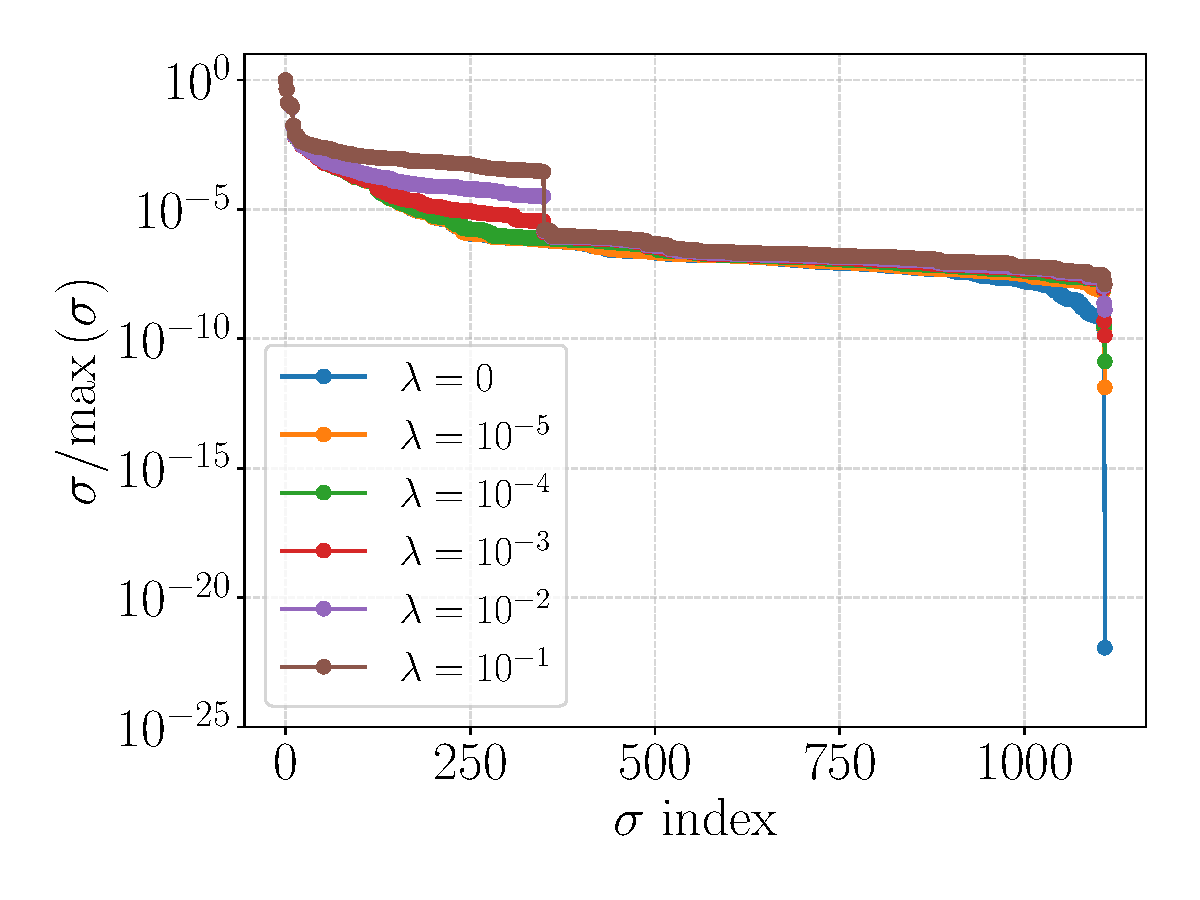
\includegraphics[width=1.0\textwidth]{figures/lm_singular_values_big_new.pdf}
    \caption{Levenberg-Marquardt.}
    \label{subfig:lm}
\end{subfigure}
 \begin{subfigure}[t]{0.49\textwidth}
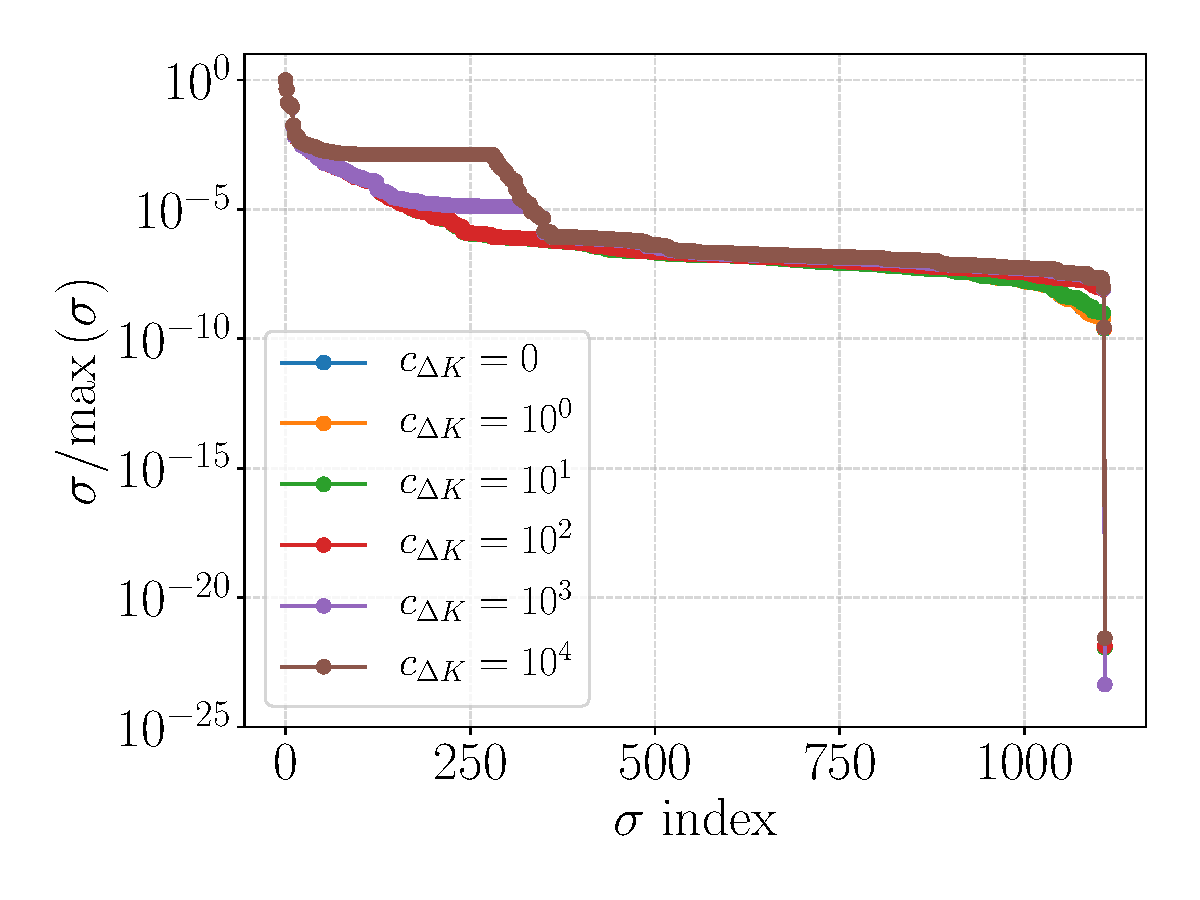
\includegraphics[width=1.0\textwidth]{figures/constraint_singular_values_big_new.pdf}
    \caption{$\Delta K$ constraint, $c_{\Delta K} = w_{\Delta K}/\sigma_{\Delta K}$.}
    \label{subfig:constraint}
\end{subfigure}
\caption{Effect of~\gls{lm} method and $\Delta K$ constraint on singular values of LOCO jacobian matrix.}
\label{fig:singval}
\end{figure}

The jacobian matrix in this analysis includes the~\gls{rf} response elements, i.e., the horizontal dispersion function is included, so the very low singular value $\sim10^{-21}$ for $\lambda = 0$ is related to the degeneracy between the vertical BPMs and correctors gains. With $\lambda = 10^{-5}$ this low singular value is already increased to $\sim10^{-12}$ and the decreasing singular values around $10^{-9}$ in the blue line are also raised. Increasing the value of $\lambda$ introduces a clear step at the $350\ts{th}$ singular value, which is related to the magnet's strengths parameters: $270$ normal quadrupoles plus $80$ skew quadrupoles. The remaining $760$ singular values are related to the BPMs and correctors parameters and their magnitude decreases very slowly. The first $12$ singular values stand out with relative strengths greater than $10^{-2}$ compared to the maximum. These values are related to the $12$ quadrupoles families and since these families are directly related to the lattice periodicity, the first $12$ singular values reflects the importance of the signature of symmetric gradient changes in the~\gls{orm}. 

In the literature~\cite{icfa_huang, huang2013}, it is recommended to start the fitting with $\lambda = 10^{-3}$. From Figure~\ref{subfig:lm} it can be seen that this value already raises the last very small singular value, avoiding the gain degeneracy problem. Increasing $\lambda$ even further introduces discontinuities in the singular values distribution, which may spoil the fitting, thus $\lambda = 10^{-3}$ really seems to be the most appropriated choice for the~\gls{lm} minimization.

Figure~\ref{subfig:constraint} shows the singular values for several constraint magnitudes. The weight vector was set as unity for every element and the normalization constant $\sigma_{\Delta K}$ was changed from $0$ to $10^{-4}$. The case $c_{\Delta K} = 0$ coincide with $\lambda = 0$ in the Figure~\ref{subfig:lm}. The normalization $\sigma_{\Delta K}$ can be interpreted as the limit of step variation in $\Delta K$. The range $0$ to $10^{-2}$ of step variation is on the order of the $K$ values for the quadrupoles and in this case the constraint does not really limits the gradients variations, which can be seen in the similar singular values distributions for $c_{\Delta K}$ from $0$ to $10^{2}$. With $c_{\Delta K}=10^{3}$ the first $350$ singular values are raised and with $c_{\Delta K}=10^{4}$ there is a clear change in the pattern at the $270\ts{th}$ singular value, which is the number of quadrupoles in the Sirius storage ring. From $270\ts{th}$ to $350\ts{th}$ a linear reduction occurs, related to the skew quadrupoles and the remaining singular values corresponds to the BPMs and correctors gains.

Limiting too much the $\Delta K$ step variation may increase unnecessarily the number of iterations required for LOCO convergence. Hence it is recommended to use the maximum value of $\sigma_{\Delta K}$ that still produces a significant change in the singular values, aiming to balance the $\Delta K$ constraints and the number of iterations, therefore reducing LOCO running time whenever it is worth it. For Sirius storage ring, the optimum value was determined to be $\sigma_{\Delta K} = 10^{-3}$, thus $c_{\Delta K} = 10^{3}$.

Notice that with $c_{\Delta K}=10^{3}$ the last singular value was smaller compared to the unconstrained case. This can be solved by combining the constrained case with the~\gls{lm} minimization, given that it was seen that the~\gls{lm} contribution raises the singular values. The singular values distribution for the chosen values of $\lambda$ and $c_{\Delta K}$ compared to the original distribution can be found in Figure~\ref{fig:compare_svs}. With this choice, the only singular value that should be removed is the last one, which is well-known to be associated with the gain degeneracy between vertical~\glspl{bpm} and correctors.
\begin{figure}
\centering
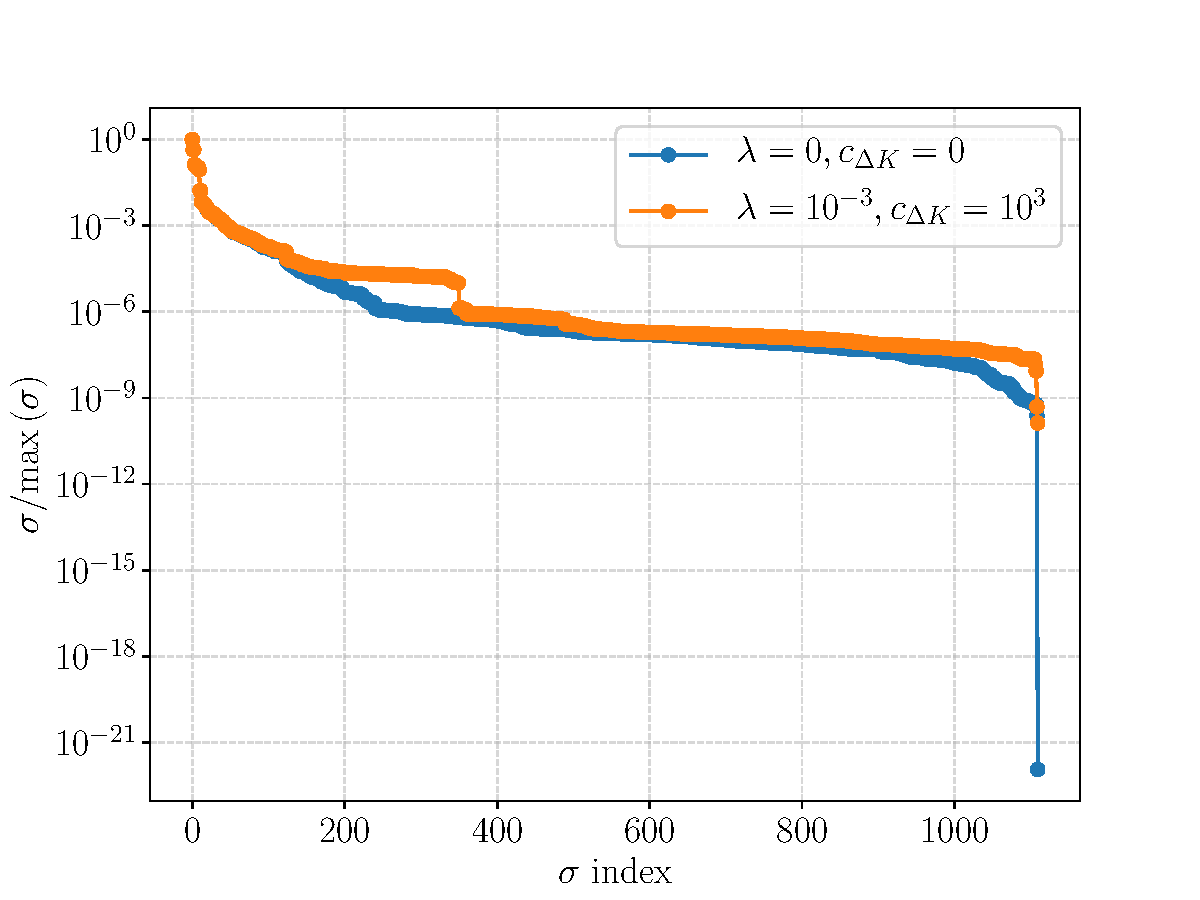
\includegraphics[width=0.75\textwidth]{figures/chosen_singular_values.pdf}
\caption{Singular values distributions between~\gls{gn} unconstrained method and~\gls{lm} constrained method with chosen parameters.}
\label{fig:compare_svs}
\end{figure}

\subsection{Detecting Distributed Errors}
The first test to check the implemented code consists in perturbing the simulated storage ring model, obtain the corresponding~\gls{orm} and then trying to determine the input errors from the fit parameters with LOCO analysis. In this way, since the planted errors perturbs the~\gls{orm} and~\gls{loco} tries to adjust the fit parameters until the goal~\gls{orm} is fitted, once the perturbed~\gls{orm} is explained by~\gls{loco}, the corresponding changes in the fit parameters should match the input errors. 

This test simulates the usage of~\gls{loco} as a diagnostic tool. However, since the only errors in the simulated model was included in the elements that was already adjusted in~\gls{loco}, subtracting the negative fit values in the perturbed model cancels out the input errors and in this way~\gls{loco} also can be viewed as a correction tool.

It is important to point out that this test should work properly if the errors are included in the elements that are used as fit parameters in LOCO method. For example, if gradient errors are added in the sextupoles but only quadrupoles strengths are fitted, the quadrupoles will be changed to best fit the~\gls{orm}. Thus, even if the $\chi^2$ is reduced, the final quadrupoles variations will not match the planted gradient errors in the sextupoles, since these elements are in different positions around the ring, with different phase advances. In this case, the fitted values must be interpreted only as the gradient changes in quadrupoles that best explain the perturbed~\gls{orm}. Clearly this type of compensation should reach a limit of fitting effectiveness. Therefore, whenever it is possible, the most appropriated approach is to identify and then to minimize the errors sources (or also called systematic errors) and, only after that, apply~\gls{loco} analysis to obtain appropriated corrections.

A hundred sets of errors were generated following a random normal distribution with $3\sigma$ cutoff. These errors were included in the simulated model and then the corresponding hundred~\gls{orm}s were calculated. LOCO analysis were performed for these~\gls{orm}s, fitting all the parameters described in Table~\ref{tab:fit_params}. The~\gls{std} $\sigma$ used in the normal distribution to generate random errors for each parameter are presented in Table~\ref{tab:errors}.
\begin{table}[h!]
    \centering
    \caption{Random errors included in the simulated model ($3\sigma$ cutoff).}
    \label{tab:errors}
    \begin{tabular}{ccc}
        \toprule\toprule
        Parameter & $\sigma$ of distribution & Unit\\ 
        \hline
        Normal quadrupole gradient & 0.1 &\% \\
        H. and V. BPM gain &  2.5 & \% \\
        H. and V. Corrector gain & 5.0 &\% \\
        Skew quadrupole gradient & $10^{-3}$ &$\SI{}{\meter^{-1}}$ \\
        % V. BPM gain &  10 & \% \\
        BPM roll angle & 10 & $\SI{}{\milli\radian}$ \\ 
        % V. Corrector gain &  10 &\% \\
        \bottomrule\bottomrule
    \end{tabular}
\end{table}

The goal of this test is to compare the fitted variations determined from~\gls{loco} with the random errors included in the model. The statistics related to the differences between these two sets of values are presented in Table~\ref{tab:diff_target}, where the difference was normalized by the~\gls{std} $\sigma$ used to generate the random errors.
% \begin{table}
%     \centering
%     \caption{Differences (normalized by $\sigma$) between planted errors and fitted variations obtained from LOCO analysis for 100 sets of random errors.}
%     \label{tab:diff_target}
%     \begin{tabular}{ccc}
%         \toprule\toprule
%         Parameter & mean difference$/\sigma$ & peak-to-valley difference$/\sigma$  \\ 
%         \hline
%         Normal quadrupole gradient & \num{9.8e-3}& $\SI{3.4e-2}{}$\\
%         H. BPM gain & $\SI{1.9e-4}{}$  & $\SI{7.9e-4}{}$\\
%         H. Corrector gain & $\SI{7.5e-5}{}$ &  $\SI{2.7e-4}{}$ \\
%         V. BPM gain & $\SI{7.7e-4}{}$ & $\SI{1.7e-3}{}$\\
%         V. Corrector gain & $\SI{7.7e-4}{}$ & $\SI{1.7e-3}{}$ \\
%         Skew quadrupole gradient & $\SI{3.9e-3}{}$  & $\SI{1.4e-2}{}$ \\
%         BPM roll angle & $\SI{3.8e-3}{}$ & $\SI{1.3e-2}{}$ \\
%         \bottomrule\bottomrule
%     \end{tabular}
% \end{table}
\begin{table}[h!]
    \centering
    \caption{Differences (normalized by $\sigma$) between planted errors and fitted variations obtained from LOCO analysis for 100 sets of random errors.}
    \label{tab:diff_target}
    \begin{tabular}{ccc}
        \toprule\toprule
        Parameter & std difference$/\sigma$ & peak-to-valley difference$/\sigma$  \\ 
        \hline
        Normal quadrupole gradient & \num{1.1e-2}& \num{5.9e-2}\\
        H. BPM gain & \num{2.8e-4} & \num{1.6e-3} \\
        H. Corrector gain & \num{1.0e-4}  & \num{5.5e-4}  \\
        V. BPM gain & \num{7.8e-4} & \num{3.2e-3} \\
        V. Corrector gain & \num{7.9e-4} & \num{3.2e-3} \\
        Skew quadrupole gradient & \num{4.9e-3} & \num{2.3e-2} \\
        BPM roll angle & \num{4.7e-3} & \num{2.2e-2} \\
        \bottomrule\bottomrule
    \end{tabular}
\end{table}

From the results in Table~\ref{tab:diff_target} it can be seen that for the normal quadrupoles, skew quadrupoles and BPM roll angles, target and obtained errors normalized by $\sigma$ agrees to within a few percent. For the gains of horizontal correctors and BPM, the difference is a few parts in ten thousand and for the vertical ones, it is a few parts in a thousand. The dispersion function was included in the fitting to break the horizontal gains degeneracy, which explains the fact that the gains determination for the horizontal plane was more efficient than the obtained in the vertical plane.
\begin{figure}
\centering
\begin{subfigure}[t]{0.49\textwidth}
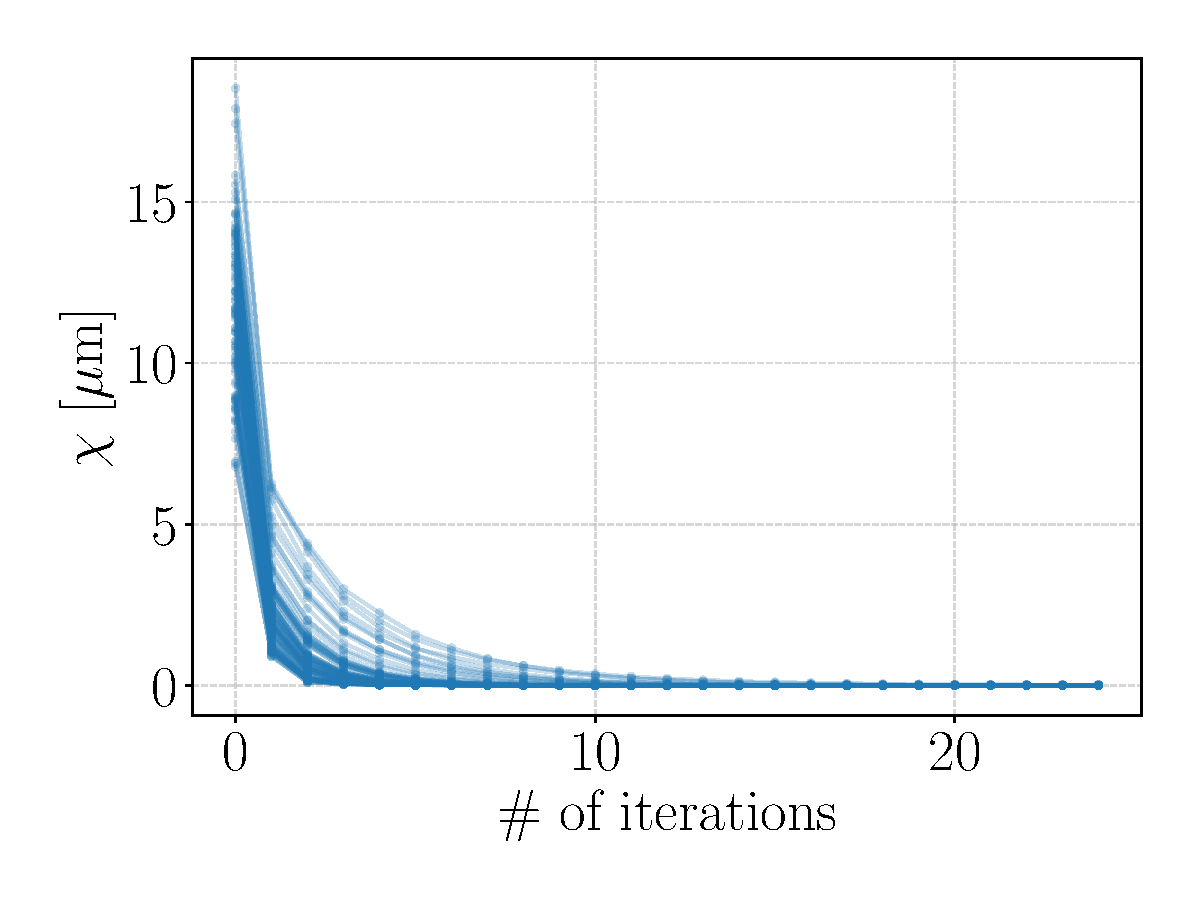
\includegraphics[width=1.0\textwidth]{figures/chi_seeds_grid_big.pdf}
    \caption{$\chi$ convergence.}
    \label{subfig:chi_seeds}
\end{subfigure}
 \begin{subfigure}[t]{0.49\textwidth}
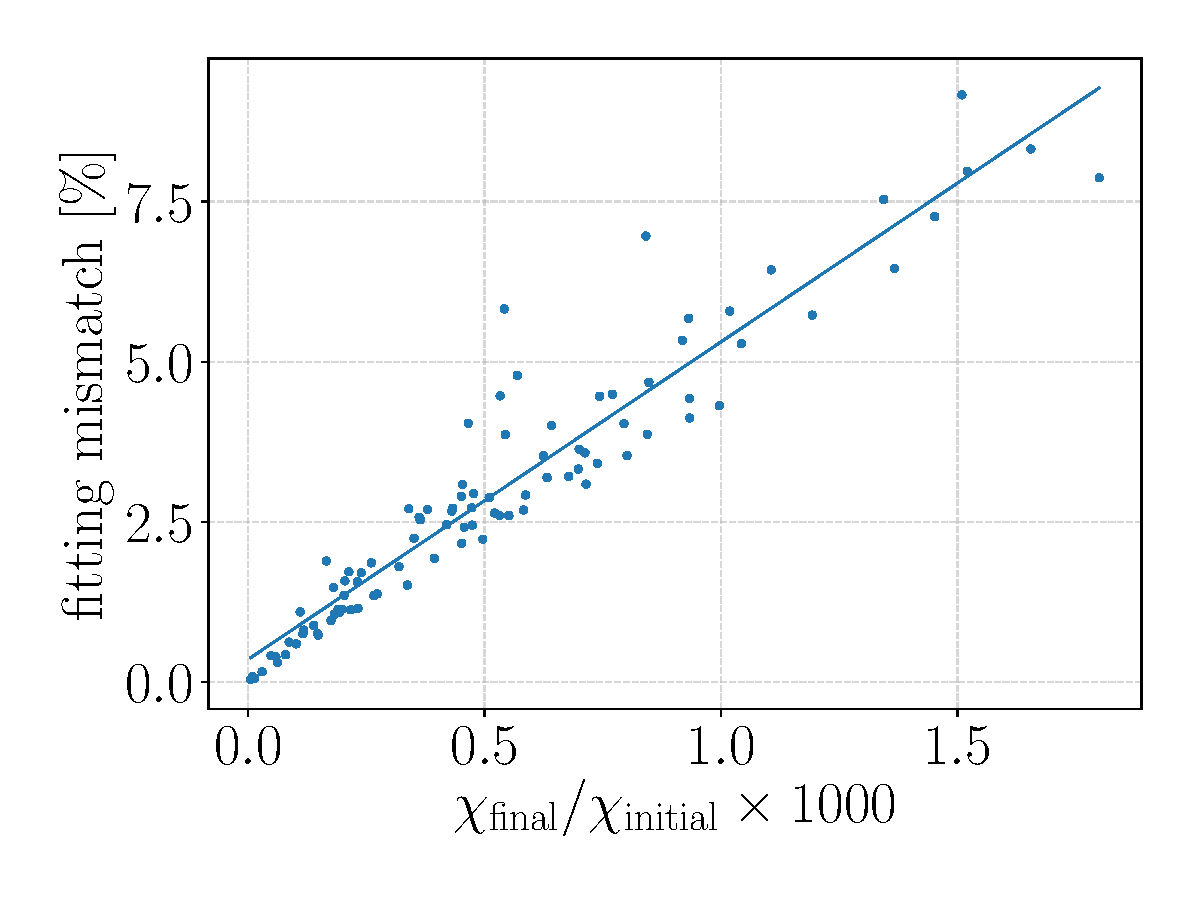
\includegraphics[width=1.0\textwidth]{figures/chi_versus_score_grid_big.pdf}
    \caption{Fitting mismatch versus fitting level.}
    \label{subfig:chi_versus_score}
\end{subfigure}
\caption{Fitting over 100 random~\gls{orm} obtained from the simulated model.}
\label{fig:fitting_seeds}
\end{figure}
The average initial $\chi$ for these 100 sets of random errors was $\SI{11.6}{\micro\meter}$ and after the fitting, the average final $\chi$ was $\SI{6.2}{\nano\meter}$. Such level of fitting is only possible because in these tests the~\gls{orm} was obtained without any noise in the data and the process is not subjected to measurement errors. For real measurements, it is desired to achieve a final value for $\chi$ that is close to the BPM accuracy, which with the current technology is typically from hundreds of nanometers to a few micrometers.

In Figure~\ref{subfig:chi_seeds} the convergence of $\chi$ for the 100 fittings is presented. The maximum number of iterations was limited to 25. It can be seen that at about 15 iterations $\chi$ already converged for all the 100 cases. Figure~\ref{subfig:chi_versus_score} shows the relation between the fitting level, represented by the ratio $\chi_{\mathrm{final}}/\chi_{\mathrm{initial}}$, and the fitting mismatch for each realization, obtained by $\sqrt{\sum_{p}d_p^2}$, where $d_p$ is the difference between target and fitted errors normalized by $\sigma$ for the parameter $p$ covering all the 7 fit parameters used in LOCO runs. The mismatch in the fitting grows linearly with the fitting level, with a proportionality factor of about 50. The code would be unreliable if the fitting level was good but the corresponding mismatch was large. Such cases were not observed in the 100 random realizations.
\subsection{Detecting Localized Errors}
Detecting single errors is very useful to identify, in a more specific way, malfunctioning elements or a problematic region in the storage ring. A functional diagnostic tool that provides this localized detection can spare a considerable amount of time in the investigation of problems that are degrading the machine performance, thus being a helpful tool for the commissioning stage and regular operation of a synchrotron light source as well, since installation and maintenance intervention occurs several times during the machine lifetime. The goal of the tests reported in the present subsection is to check LOCO ability to identify localized errors on quadrupoles, BPMs and correctors. 

\subsubsection{Single Gradient}
Suppose that amongst random gradient errors in quadrupoles, there is a single quadrupole with a large deviation from its nominal value. Single quadrupole errors are not naturally expected, since magnetic measurements are performed before the assembly in storage ring to guarantee that mechanical and magnetic properties meet the specifications for all magnets. However, after the magnets assembly some kind of problem in a specific magnet coils or in its power supply may appear and lead to localized errors.

The following error distribution was generated and applied in Sirius storage ring model: gaussian random errors in gradient strengths with std $\sigma=\SI{0.25}{\%}$ and $\SI{2.0}{\%}$ of error in the 215\ts{th} quadrupole. Errors in others parameters were not included. An~\gls{orm} was calculated with this perturbed model and it was used as input for LOCO analysis, including all fit parameters. The results for variations in quadrupoles fitted by LOCO compared to the target errors are in Figure~\ref{fig:single_quad_detec}.
\begin{figure}[h!]
\centering
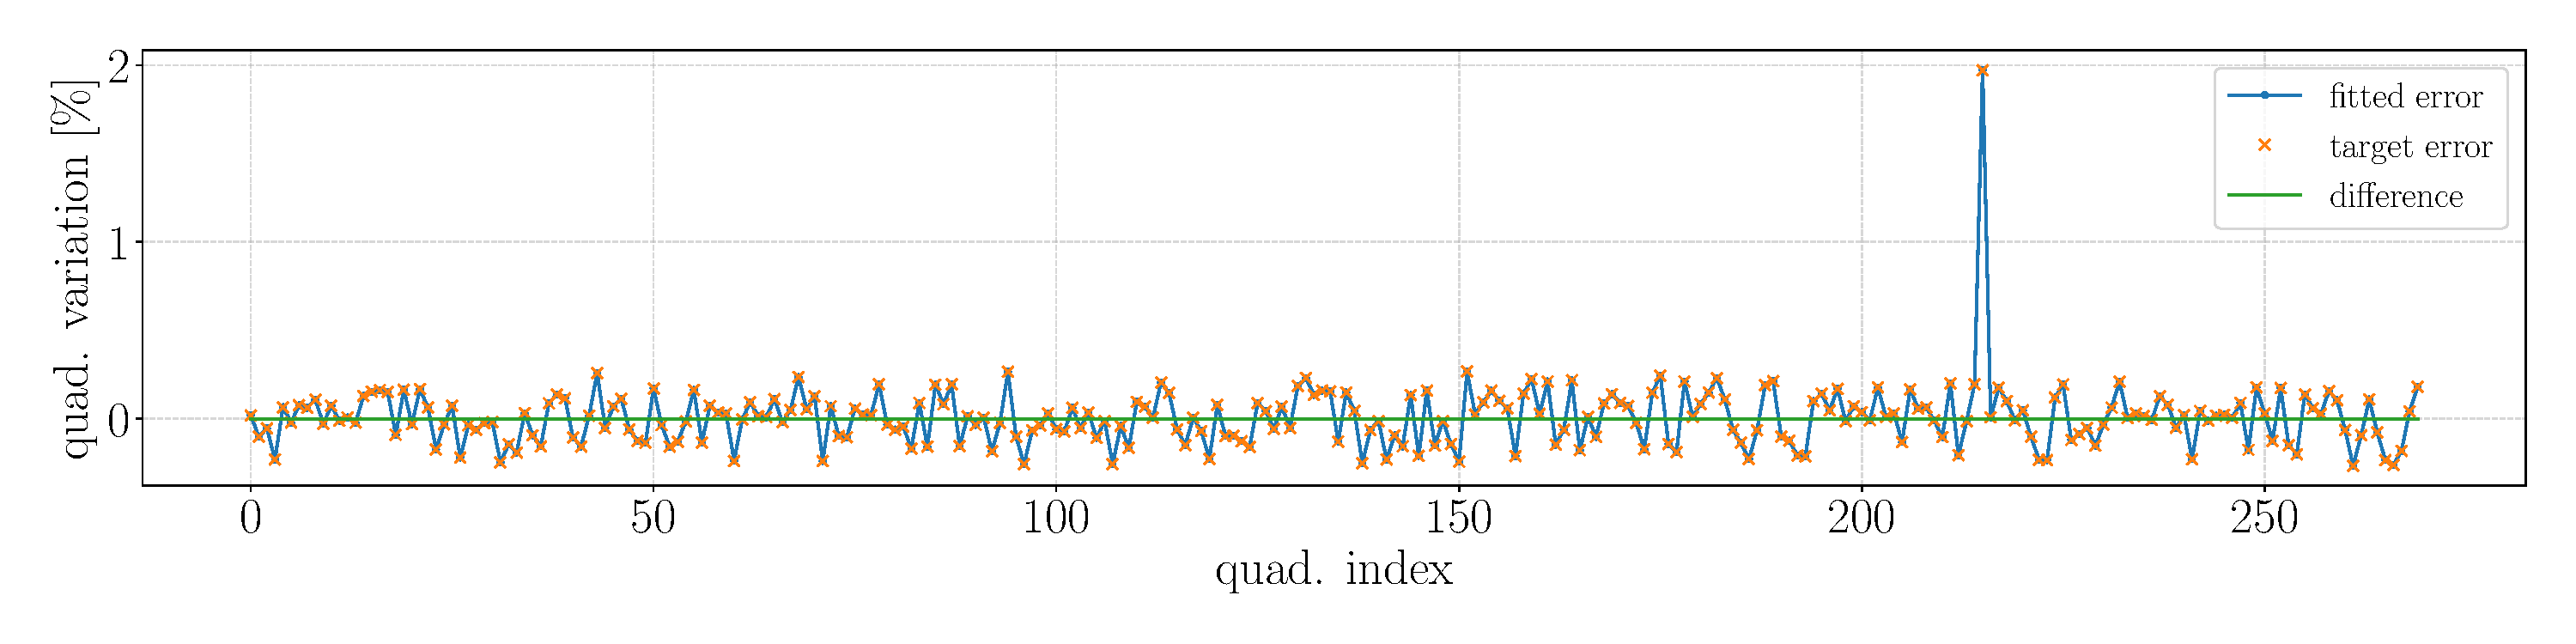
\includegraphics[width=1.0\textwidth]{figures/single_quaderror_detection_big.pdf}
\caption{Fitted and target quadrupoles variations, including a higher error of 2\% in the 215\ts{th} quadrupole.}
\label{fig:single_quad_detec}
\end{figure}

From Figure~\ref{fig:single_quad_detec} it can be seen that the input errors were accurately determined, including the single large gradient error. The maximum difference between fitted and target error for quadrupoles was $\num{1e-8}$. The final value of $\chi$ in this fitting was very low, around $\SI{1e-6}{\micro\meter}$. The variations on the remaining fit were in a much lower level, the maximum variation of BPM gains and correctors was $\num{3e-6}$ and for skew quadrupoles strengths $\SI{1e-16}{\meter^{-1}}$, on the order of computer numeric precision.

It is clear that this level of error determination is only possible for tests in the simulated model, when the goal~\gls{orm} was obtained without noise and measurement errors. Nevertheless, in the limit that these practical limitations are set as low as possible in real measurements, it would still be possible to identify single errors with reasonable accuracy.
\subsubsection{Single Gain}
The same tests were performed with BPMs and correctors gains. Such type of error in gains may be associated with malfunctioning in~\glspl{bpm} antennas, electrical interference or software issues. For correctors the outliers in gains may indicate problems in the magnet coils or in its power supplies. For BPMs, the problems are typically easier to detect since they can be identified directly from unrealistic position measurements. For correctors, the effect on the beam produced by localized problems may be more subtle to identify directly. Measuring the~\gls{orm} and performing LOCO analysis is usually a good indirect procedure to detect the aforementioned errors.

Gaussian random errors with std $\sigma=\SI{10}{\%}$ were applied both for horizontal and vertical gains. BPM roll angle errors were included following a gaussian random distribution with std $\sigma=\SI{1}{\milli\radian}$.  The corresponding gains for 7\ts{th} BPM, CH and CV were increased by a $1.5$ factor. This means that the nominal~\gls{orm}, after applying the random gains errors, had the 7\ts{th} and 167\ts{th} rows (for the 7\ts{th} BPM) and 7\ts{th} and 127\ts{th} columns (for the 7\ts{th} CH and CV) multiplied by $1.5$. This altered~\gls{orm} were set as the goal matrix for LOCO fitting, where all fit parameters were included again. The fitting results for this test are shown in Figure~\ref{fig:gain_greater}.
\begin{figure}[h!]
\centering
\begin{subfigure}[t]{0.49\textwidth}
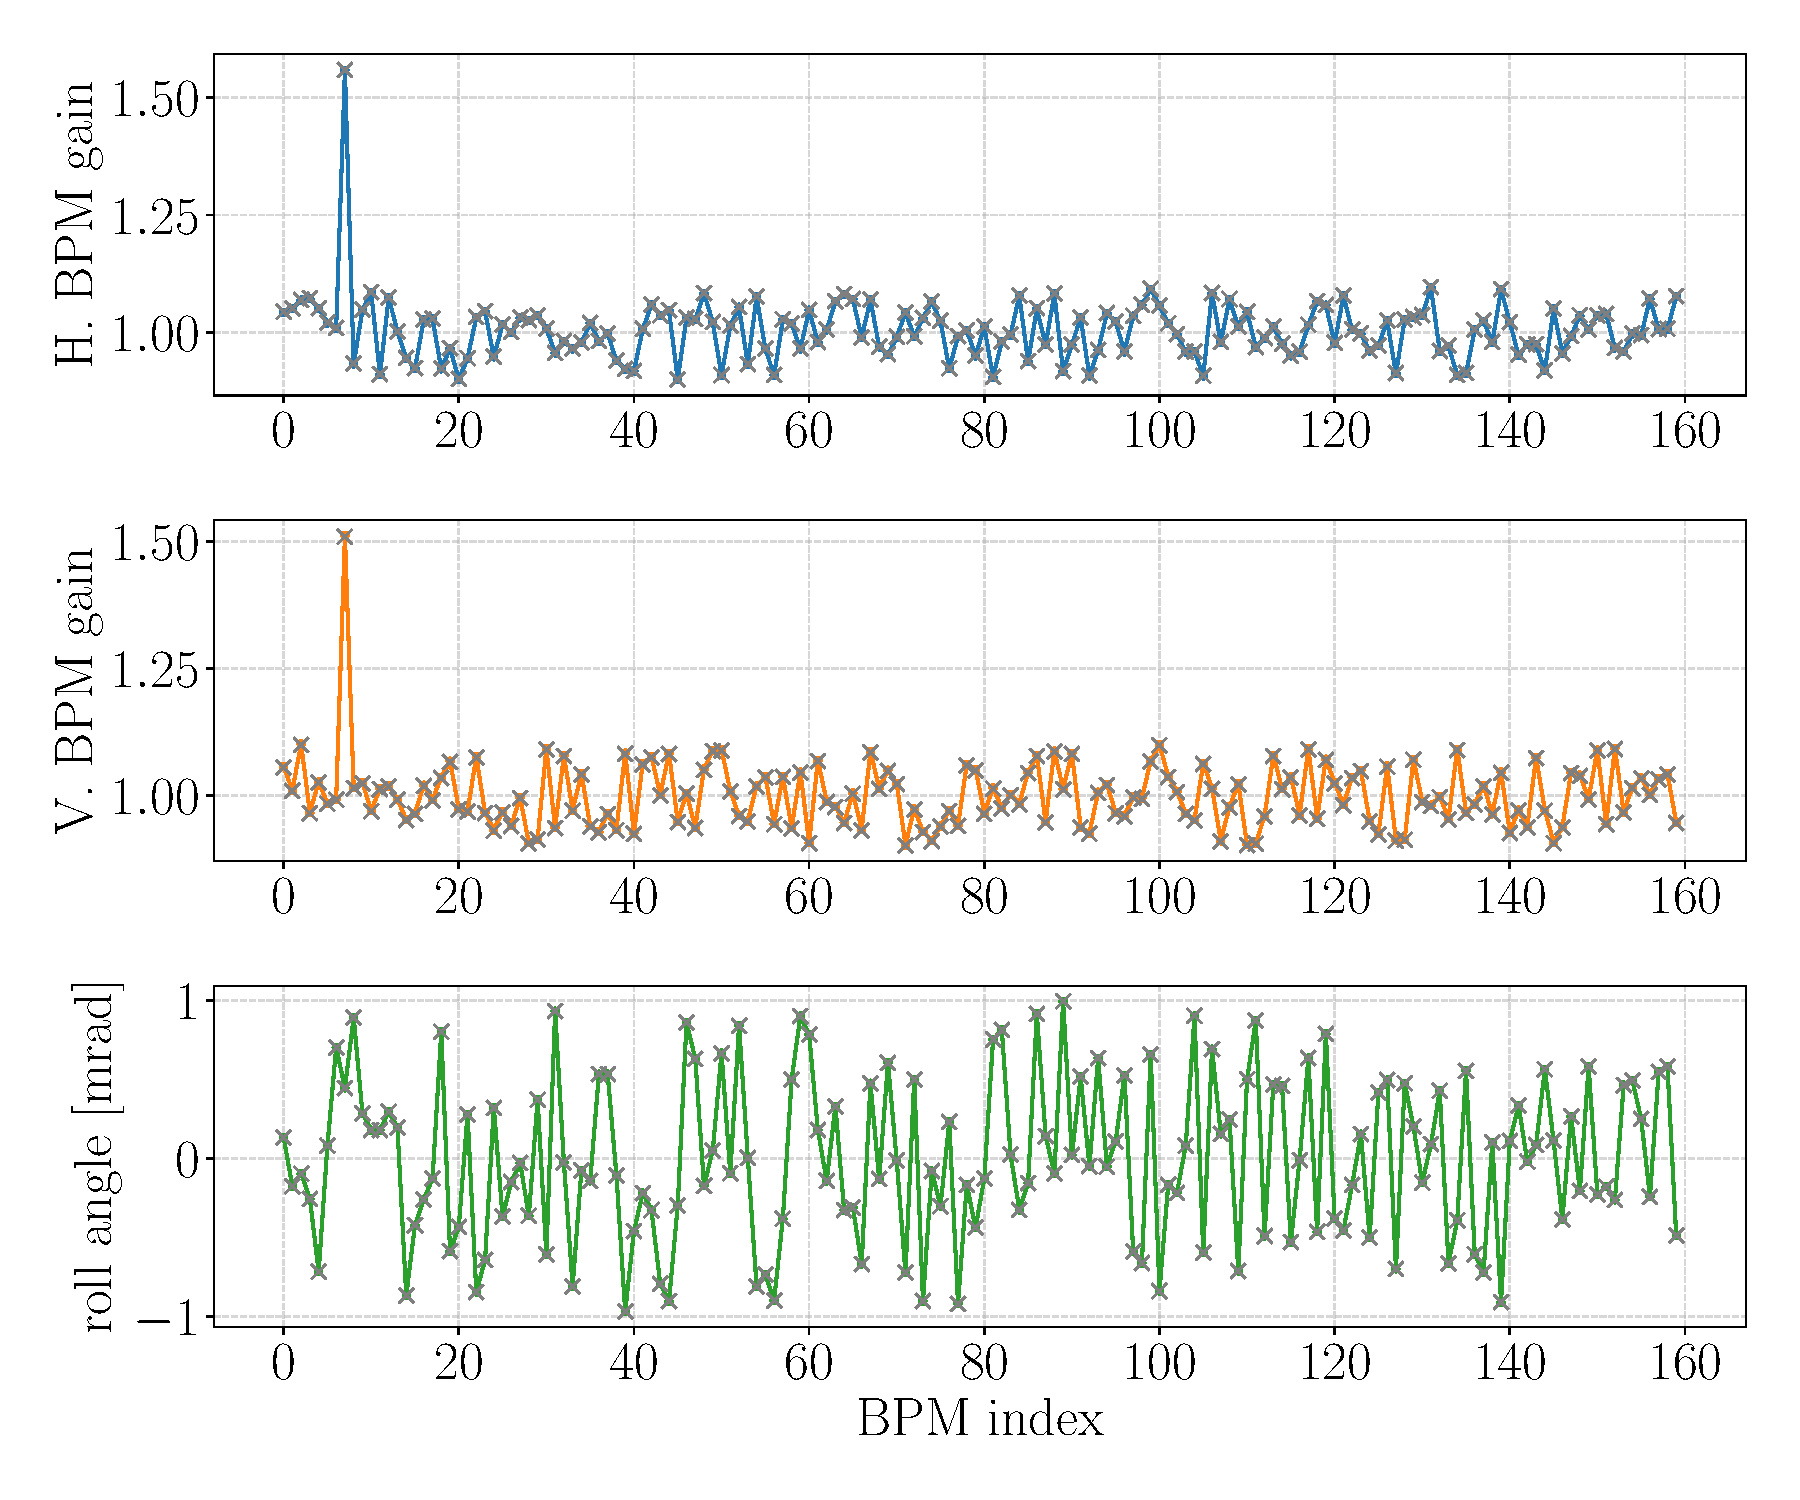
\includegraphics[width=1.0\textwidth]{figures/bpm_gains_1p5gain_7th_bpm_grid_big.pdf}
    \caption{BPM gains and roll angles.}
    \label{subfig:bpm_fit_gain_greater}
\end{subfigure}
 \begin{subfigure}[t]{0.49\textwidth}
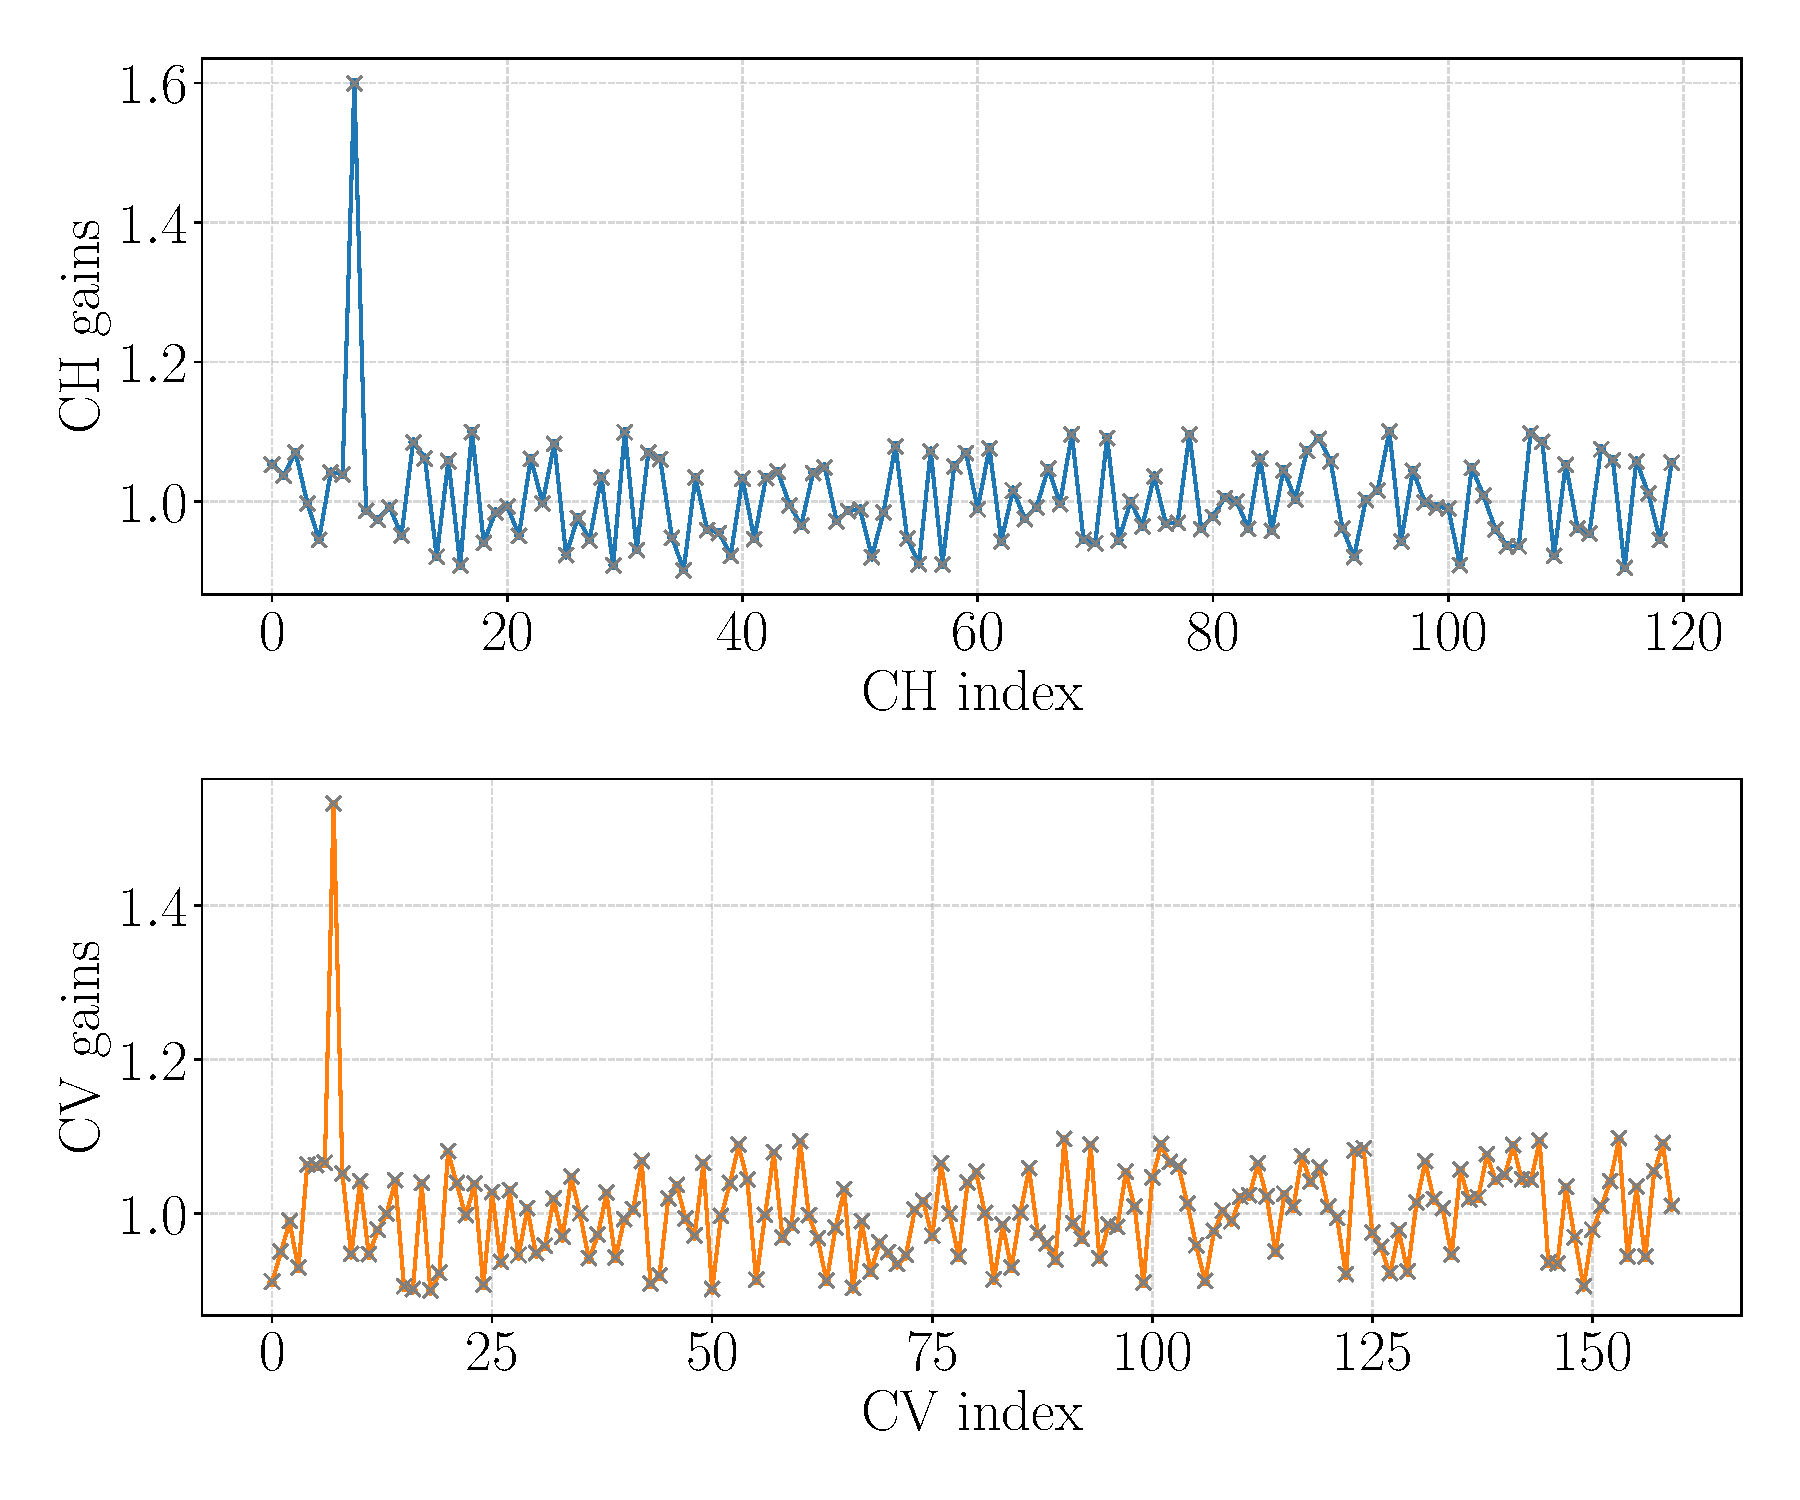
\includegraphics[width=1.0\textwidth]{figures/corr_gains_chcv_1p5_grid_big.pdf}
    \caption{Correctors gains.}
    \label{subfig:corr_fit_gain_greater}
\end{subfigure}
\caption{Fitted values for BPM gains, roll errors and correctors (CH and CV) gains, where the 7\ts{th} BPM, CH and CV gains are greater by a 1.5 factor. Gray $\times$ represents the target errors.}
\label{fig:gain_greater}
\end{figure}

Once again, the input errors were determined precisely and the larger planted gains were identified, both for BPM and correctors. The maximum difference between fitted and target error for horizontal gains (BPM and CH) was $\SI{0.2}{\%}$ and for vertical gains (BPM and CV) was $\SI{0.1}{\%}$. The other parameters were changed again in a lower level, the maximum variation for quadrupoles was $\SI{2e-6}{}$ and for skew quadrupoles $\SI{4e-9}{\meter^{-1}}$.

% \subsubsection{Elements Swap}
% The last test regarding localized errors detection is swapping of elements in a storage ring. Even tough the elements installation and communication with the control system are performed and checked carefully, due to the large number of devices, some errors may remain. This type of problem may be found mainly in early commissioning stages. However, interventions in the devices, for maintenance, elements replacement or software updates in the control system, may produce a non-zero chance of element swapping. A quite common type of devices swapping found in storage ring is related to BPMs, in cables or in control system. 

%~\gls{bpm} and correctors swap can be simulated simply by swapping the corresponding~\gls{orm} rows and columns. To simulate an exchange between 6\ts{th} and 7\ts{th} BPM, the nominal~\gls{orm} had its 6\ts{th} and 166\ts{th} rows swapped with 7\ts{th} and 167\ts{th} rows and this manipulated matrix was set as input for LOCO. In this way it was simulated only the effect of element swap, since all the fit parameters are exactly equal to the nominal values. 

% The initial $\chi$ between swapped~\gls{bpm} matrix and the nominal one in this case was $\SI{15}{\micro\meter}$. The LOCO realized only 2 iterations, reducing only to $\chi = \SI{2.3}{\micro\meter}$, i.e., the goal matrix could not be explained in a typical fitting level. In Figure~\ref{fig:swap_bpm}, the gains obtained from this fitting are presented.
% \begin{figure}
% \centering
% 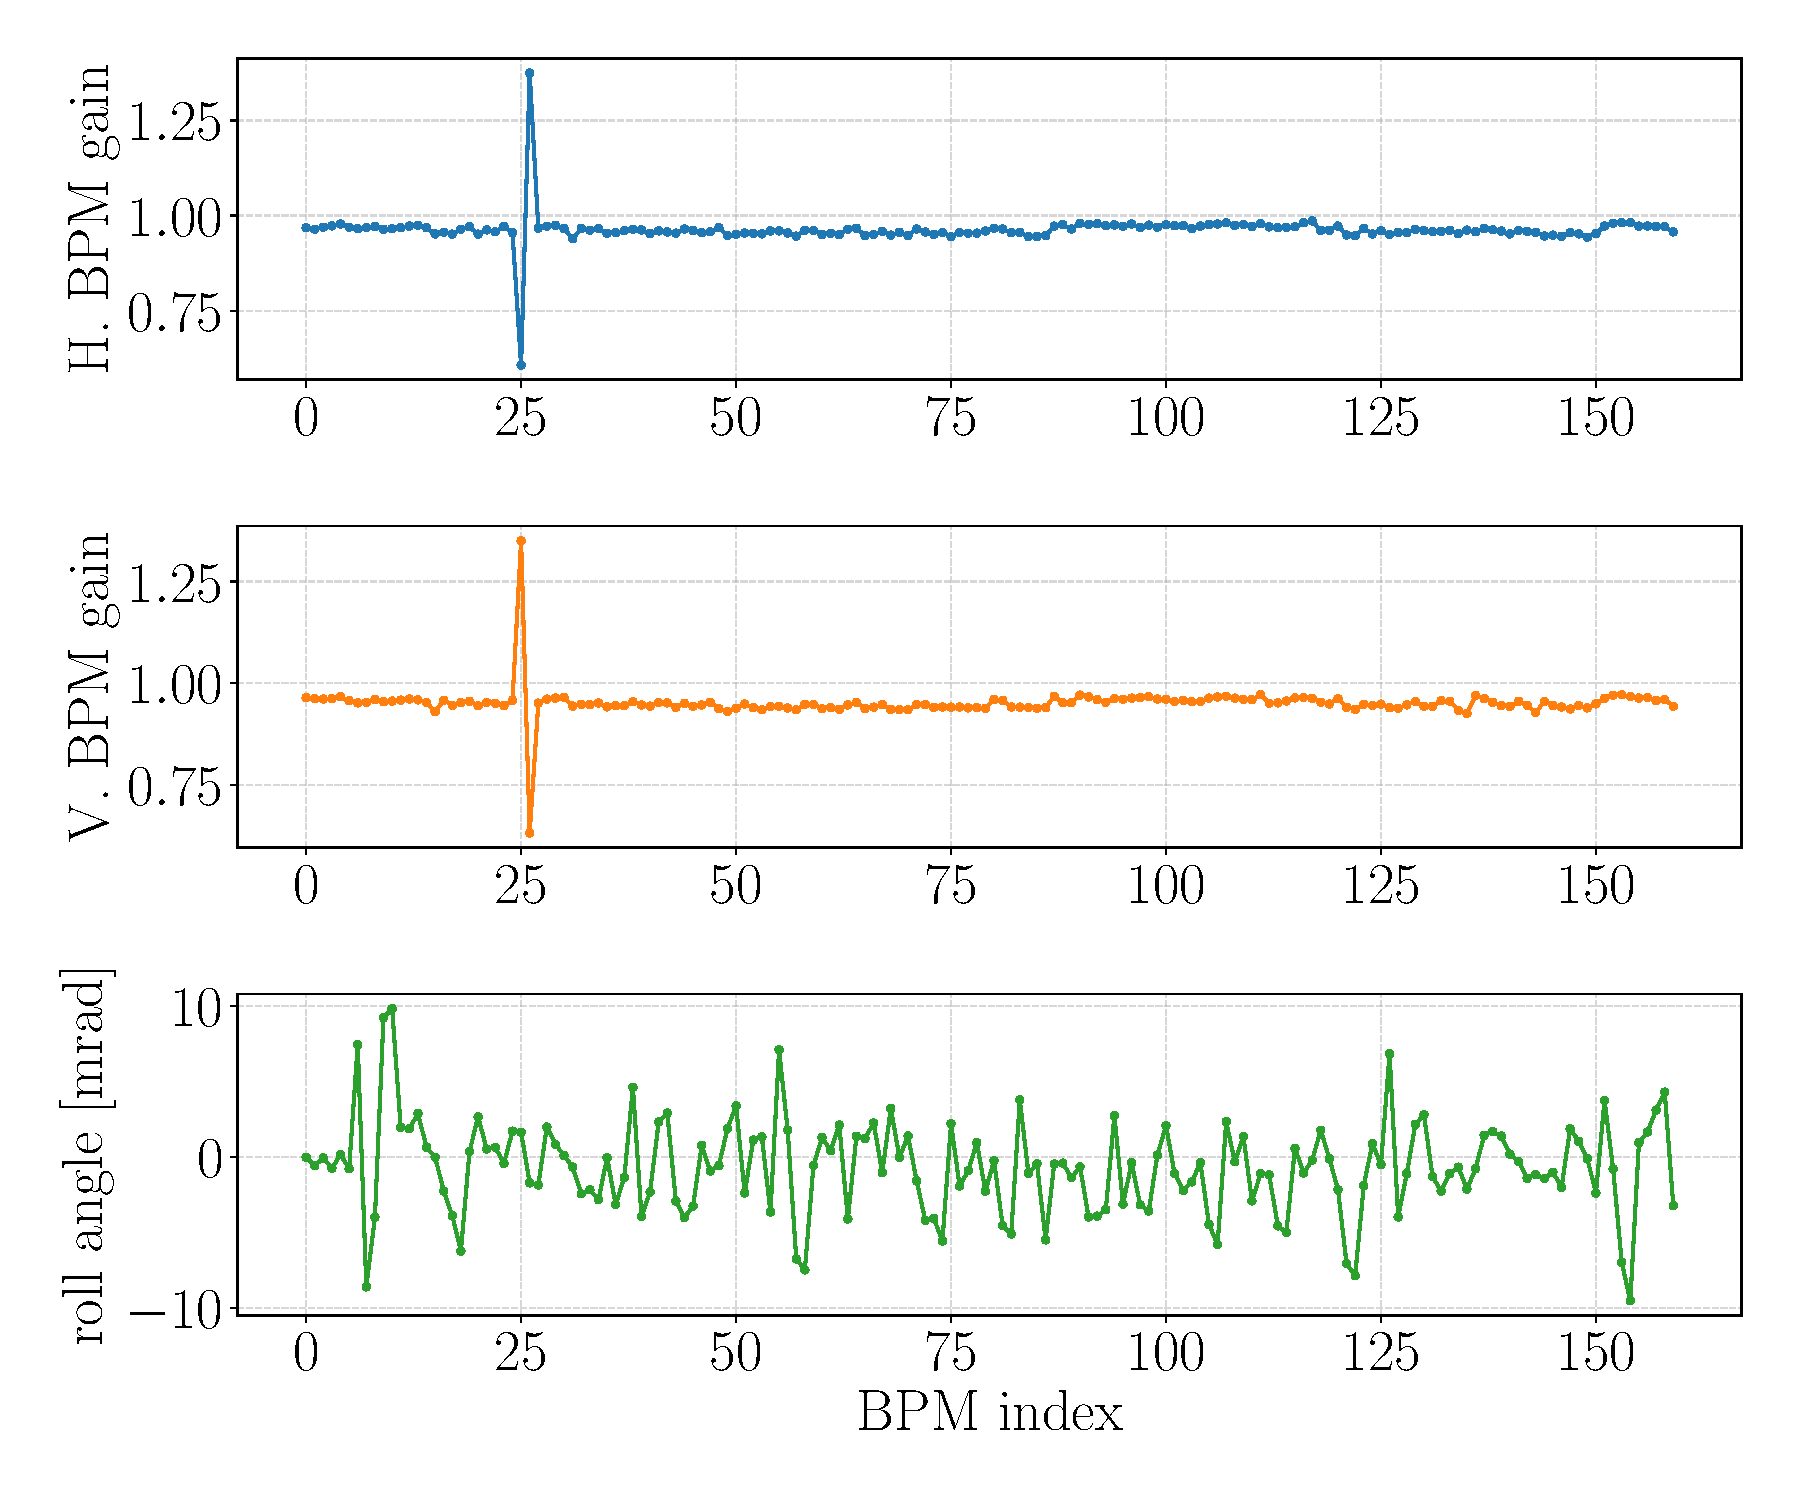
\includegraphics[width=1.0\textwidth]{figures/corr_gains_swap_bpm_25_26.pdf}
% \caption{25\ts{th} and 26\ts{th} BPMs}
% \label{fig:swap_bpm}
% \end{figure}

% % \begin{figure}
% % \centering
% % \begin{subfigure}[t]{0.49\textwidth}
% % 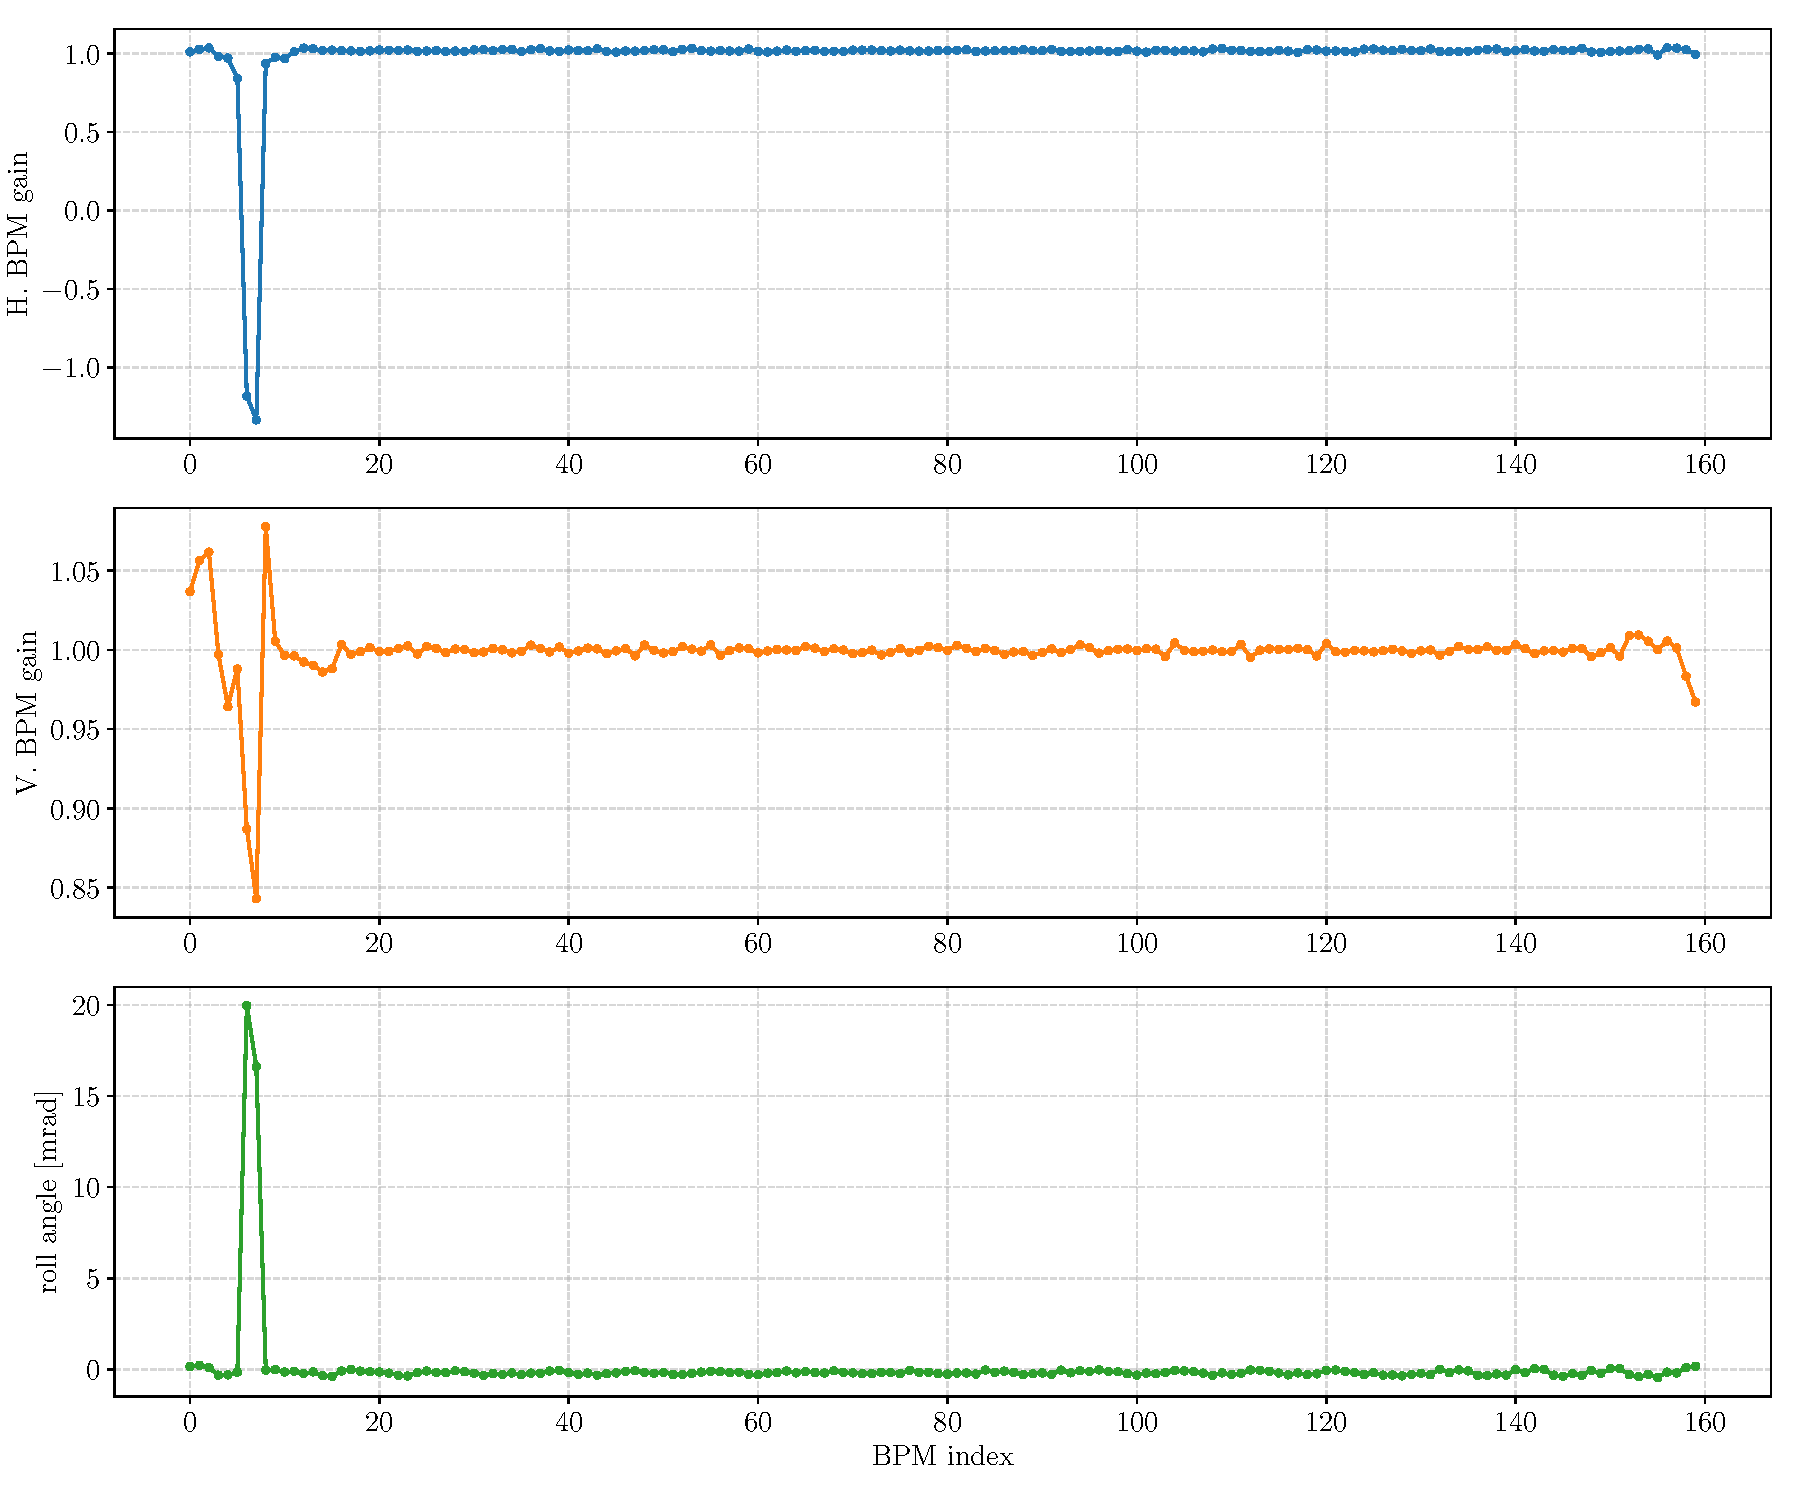
\includegraphics[width=1.0\textwidth]{figures/bpm_gains_swap_6with7_grid.pdf}
% %     \caption{BPM gains and roll angles.}
% %     \label{subfig:bpm_fit_swap_bpm}
% % \end{subfigure}
% %  \begin{subfigure}[t]{0.49\textwidth}
% % 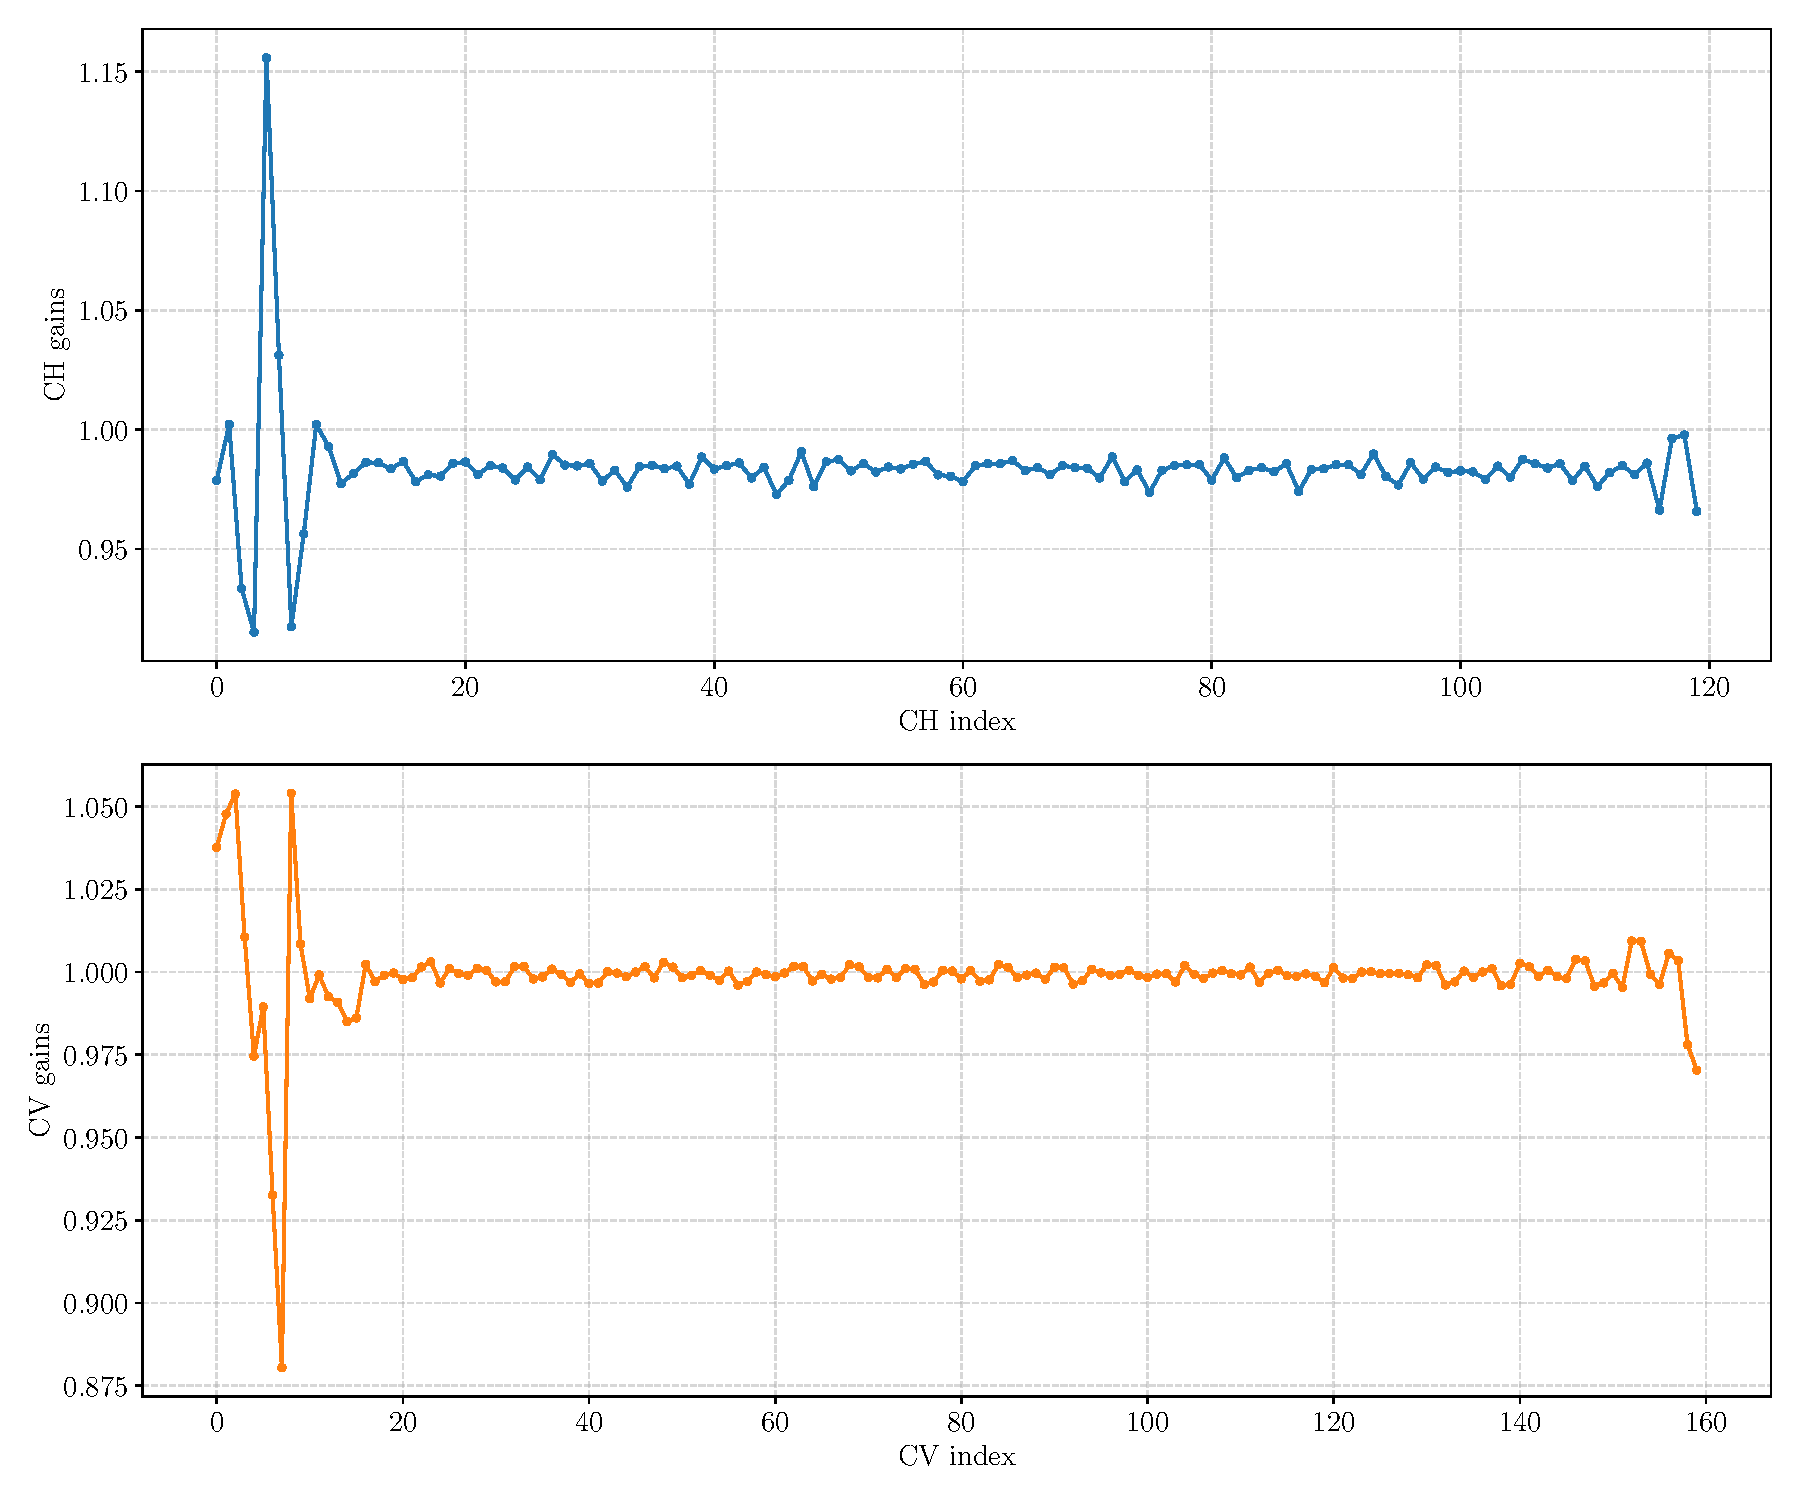
\includegraphics[width=1.0\textwidth]{figures/corr_gains_bpm_swap_6with7_grid.pdf}
% %     \caption{Correctors gains.}
% %     \label{subfig:corr_fit_swap_bpm}
% % \end{subfigure}
% % \caption{Fitted values for BPM gains, roll errors and correctors (CH and CV) gains swapping 6\ts{th} and 7\ts{th} BPMs.}
% % \label{fig:swap_bpm}
% % \end{figure}

% In adjusted BPMs gains and roll angles it can be clearly identified that the values for 6\ts{th} and 7\ts{th} stand out compared the remaining BPMs, even reaching negative horizontal gains. CH and CV gains near the region where the swap was performed also indicate that this region is problematic. These obvious outliers, especially the unrealistic horizontal gains, can be used to point out that there is a type of o problem in 3\ts{rd} and 2\ts{nd} BPMs that can not be explained with transformations of scales and rotations. 

% To simulate an exchange between 6\ts{th} and 7\ts{th} CHs, the nominal~\gls{orm} had its 6\ts{th} column swapped with 7\ts{th}. LOCO method was applied using this changed matrix as goal. Once again, the convergence was stopped after 2 iterations, with $\chi$ reduced from $\SI{15.5}{\micro\meter}$ to $\SI{4.6}{\micro\meter}$, indicating a worse fitting level compared to the one obtained in BPM swap. The fitted gains in this test are shown in Figure~\ref{fig:swap_ch}.
% \begin{figure}
% \centering
% \begin{subfigure}[t]{0.49\textwidth}
% 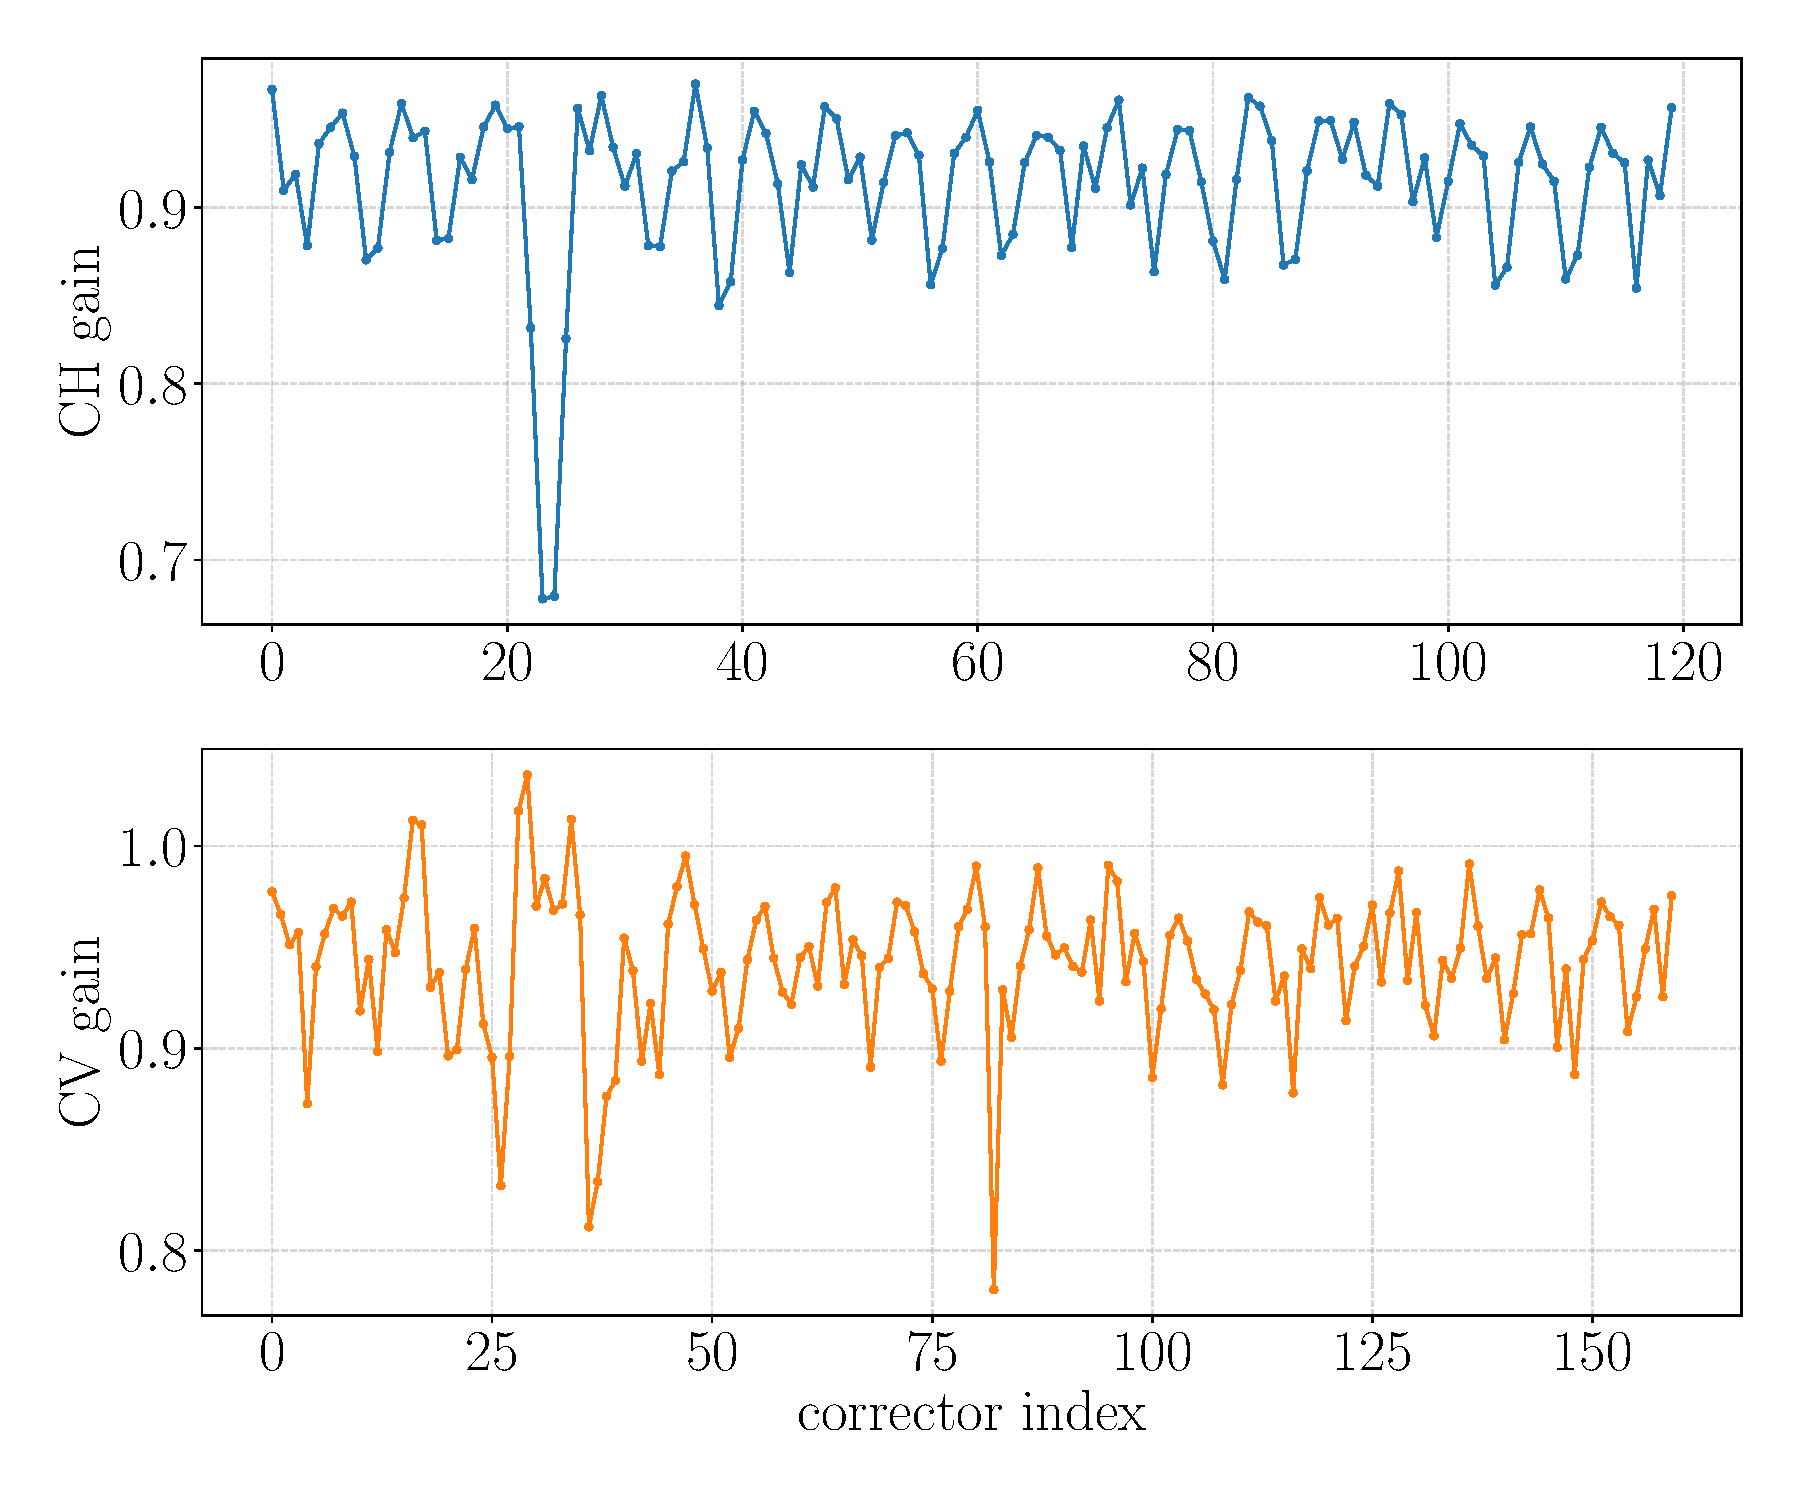
\includegraphics[width=1.0\textwidth]{figures/corr_gains_swap_ch_23_24.pdf}
%     \caption{CH swap.}
%     \label{subfig:bpm_fit_swap_ch}
% \end{subfigure}
%  \begin{subfigure}[t]{0.49\textwidth}
% 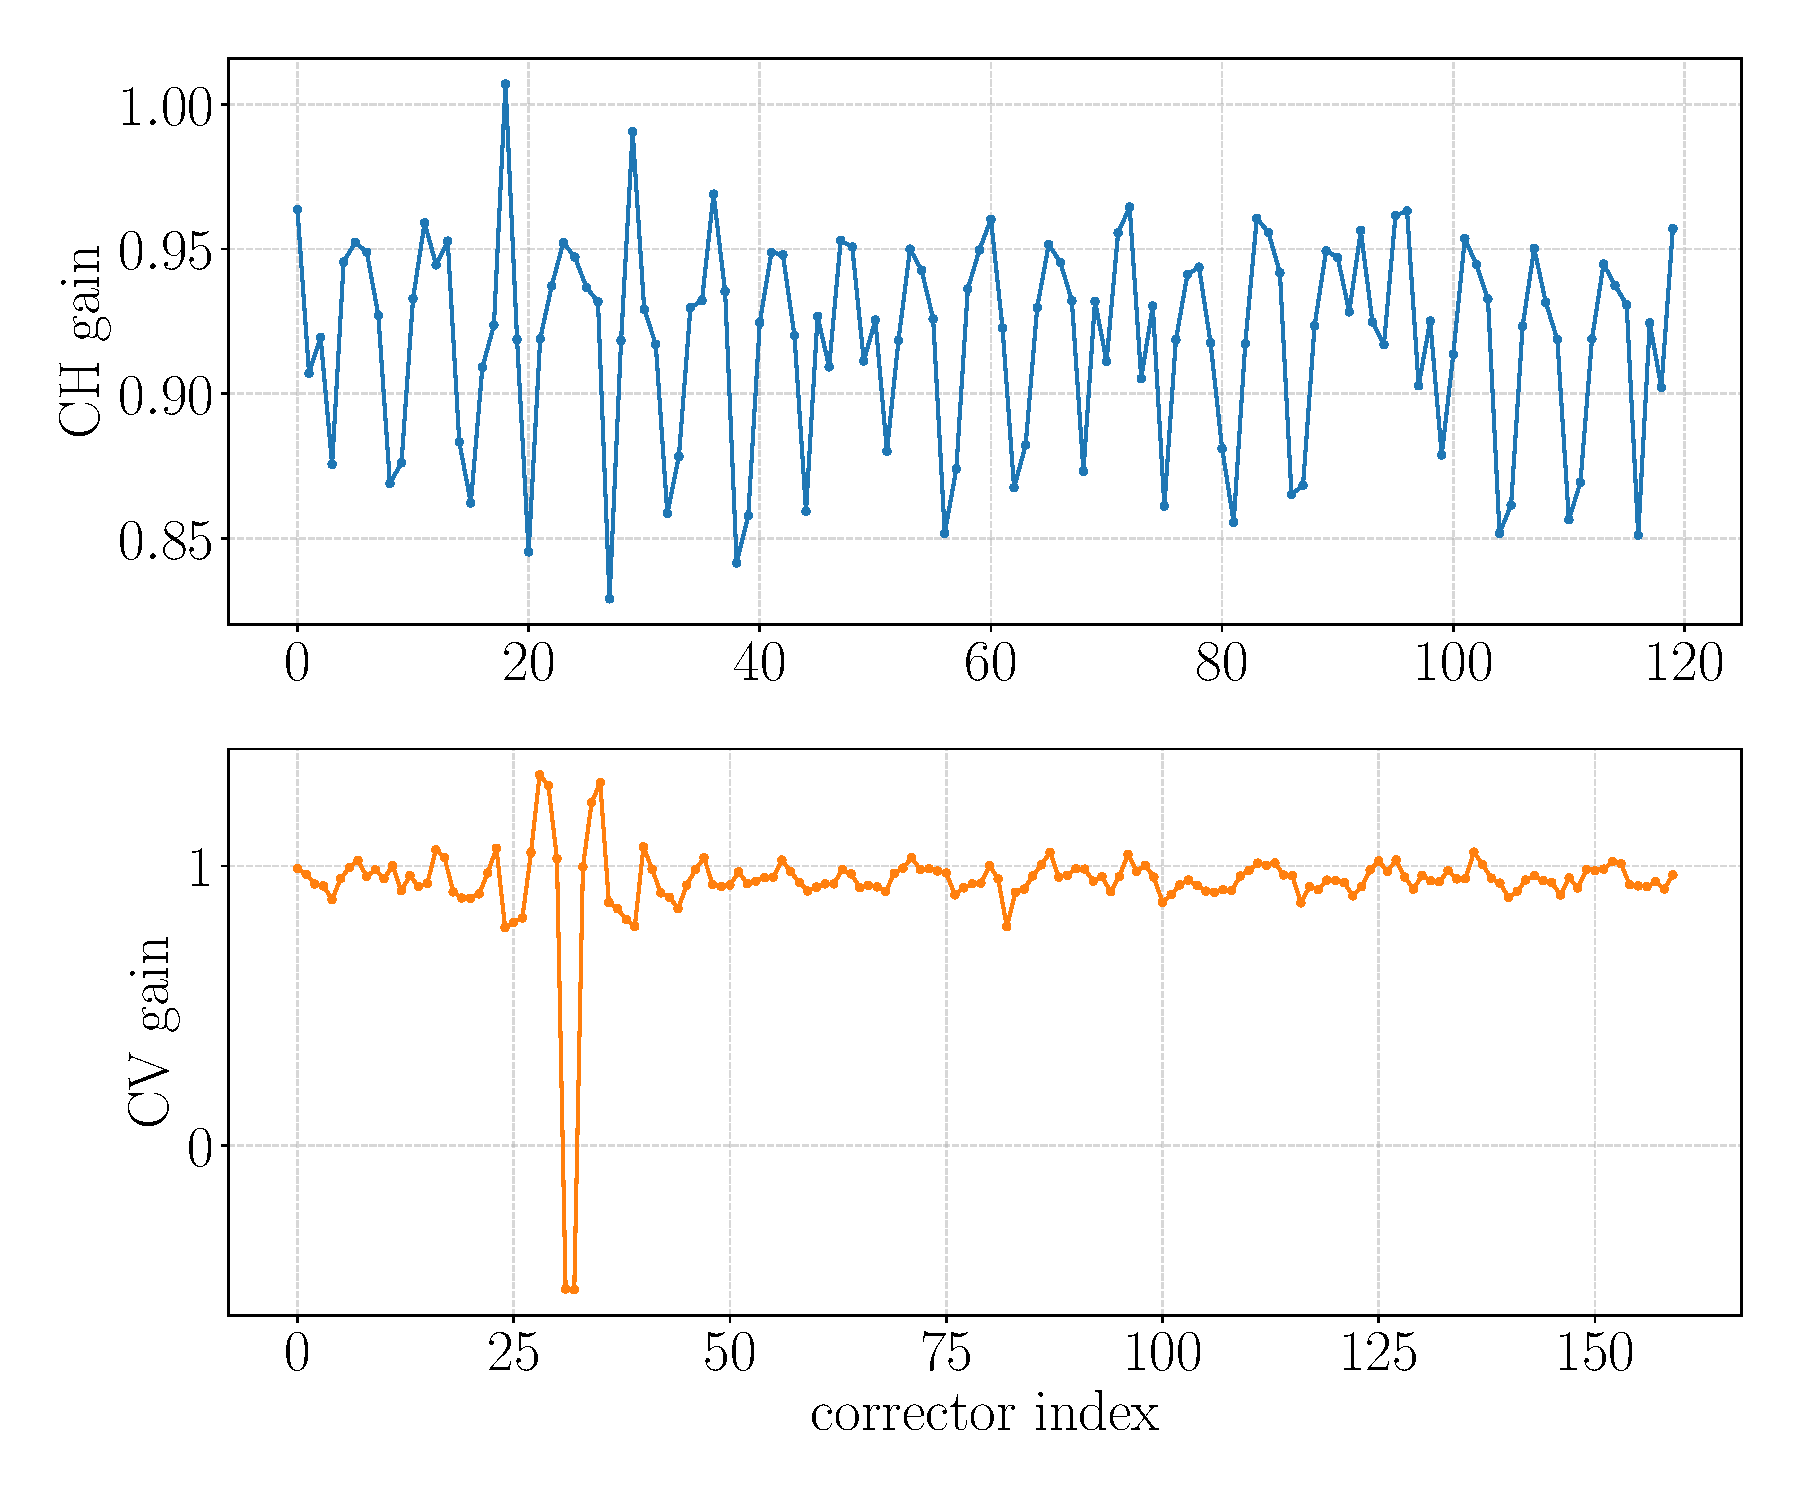
\includegraphics[width=1.0\textwidth]{figures/corr_gains_swap_cv_31_32.pdf}
%     \caption{CV swap.}
%     \label{subfig:corr_fit_swap_cv}
% \end{subfigure}
% % \caption{Fitted values for BPM gains, roll errors and correctors (CH and CV) gains swapping 6\ts{th} and 7\ts{th} CHs.}
% \label{fig:swap_corr}
% \end{figure}

% In adjusted gains for CH, the values for 6\ts{th} and 7\ts{th} horizontal correctors surely differ from the remaining values, reaching negative values as well. The other fitted gains around the swap region are also disturbed. The same behavior is valid for CV swapping, affecting the vertical corrector gains.

% With the studies performed with elements swapping in~\gls{orm}, one can conclude that, even for discontinuous errors like this, the LOCO method can still provide useful information. The unrealistic fitted gains in the elements may indicate that there is a localized discrepancy between the lattice that generated the goal~\gls{orm} and the model lattice that had its parameters varied to fit the goal matrix. Since the LOCO method applies linear transformations (scales changes with gains and rotations with roll angles) in~\gls{orm}, transformations like rows and columns exchanges can not be covered. 

% Nevertheless, if this behavior is observed in LOCO analysis performed with measured~\glspl{orm}, one has evidences of localized problems that can be investigated more efficiently. For example, based on the localized negative gains, one can swap the corresponding rows or columns in nominal~\gls{orm} and compare the signatures with measured~\gls{orm}. Since unguided searching for problems in such a complex system as a storage ring with thousands of elements is clearly impractical, a tool that may reduce the search space dimensions is very valuable for machine operation, on the commissioning context and on the regular basis as well, after machine maintenance events, for example.

